\chapter{Supplementary Material for Chapter 5: RankGen}
\label{appendix:ch5}
\label{app:theory-metric-defs}


\label{appendix:bounds}

\begin{table}[H]
\centering

\label{tab:notation-glossary}
\vspace{-1.5em}

\footnotesize
\setlength{\tabcolsep}{5pt}
\renewcommand{\arraystretch}{1}

\resizebox{\textwidth}{!}{%
\begin{tabular}{@{}p{3.1cm}p{2.2cm}p{9.2cm}@{}}
% \toprule
\textbf{Symbol} & \textbf{Type} & \textbf{Meaning / definition} \\
\midrule

\multicolumn{3}{@{}l}{\emph{Datasets and sample sizes}}\\
$D_{\text{train1}}^{(i)}$ & set & Real training subset used for the baseline classifier.\\
$D_{\text{train2}}^{(i)}$ & set & Additional real data used for the upper-bound classifier.\\
$D_{\text{generated}}^{(i)}$ & set & Generated data produced by the generator.\\
$D_{\text{test}}$ & set & Held-out real test set used for evaluation.\\
$D_{\mathrm r},\;D_{\mathrm g}$ & sets & Real and generated sample sets in the similarity setting.\\
$D_{\text{mix}}^{(i)}$ & set & Mixed pool $D_{\text{train1}}^{(i)} \cup D_{\text{generated}}^{(i)}$ used to measure local mixing.\\
$n,\;n_r,\;n_g$ & scalars & Total, real, and generated sample sizes, with $n=n_r+n_g$.\\
$m$ & scalar & Size of the balanced discriminator/domain-classifier pool.\\
$k$ & scalar & Number of nearest neighbours in the similarity metric.\\
$P_r,\;P_g$ & distributions & Real data distribution and generated data distribution.\\

\midrule
\multicolumn{3}{@{}l}{\emph{Model classes}}\\
$\Phi_\theta$ & map & Task classifier architecture.\\
$\Psi_\theta$ & map & Real-vs-generated discriminator.\\
$\Gamma_\theta$ & map & Helper used to compute the similarity statistic.\\

\midrule
\multicolumn{3}{@{}l}{\emph{Raw classifier accuracies}}\\
$\rho_1^{(i)}$ & num. & Task score using $\Phi_\theta$ trained on $D_{\text{train1}}^{(i)}$ only.\\
$\rho_2^{(i)}$ & num. & Task score using $\Phi_\theta$ trained on $D_{\text{generated}}^{(i)}$ only.\\
$\rho_3^{(i)}$ & num. & Task score using $\Phi_\theta$ trained on $D_{\text{train1}}^{(i)} \cup D_{\text{train2}}^{(i)}$.\\
$\rho_4^{(i)}$ & num. & Task score using $\Phi_\theta$ trained on $D_{\text{train1}}^{(i)} \cup D_{\text{generated}}^{(i)}$.\\
$\rho_5^{(i)}$ & num. & Discriminator accuracy for distinguishing real from generated samples.\\
$\rho_6^{(i)}$ & num. & Raw similarity statistic used to construct $S^{(i)}$.\\
$\rho_j^\star$ & num. & Population counterpart of $\rho_j^{(i)}$.\\

\midrule
\multicolumn{3}{@{}l}{\emph{Derived quantities}}\\
$\Delta_{\text{real}}^{(i)}$ & num. & $\rho_3^{(i)}-\rho_1^{(i)}$, gain from adding more \emph{real} data.\\
$\Delta_{\text{generated}}^{(i)}$ & num. & $\rho_4^{(i)}-\rho_1^{(i)}$, gain from adding \emph{generated} data.\\
$\gamma^\star$ & num. & $|R_Q(h_s)-R_Q(h_{r'})|$, generated-domain gap between $h_s$ and $h_{r'}$.\\
$Q^{(i)}$ & num. & Empirical quality score on split $i$.\\
$Q^\star$ & num. & Population quality score.\\
$U^{(i)}$ & num. & Empirical utility score on split $i$.\\
$U^\star$ & num. & Population utility score.\\
$I^{(i)}$ & num. & Empirical indistinguishability score on split $i$.\\
$I^\star$ & num. & Population indistinguishability score.\\
$S^{(i)}$ & num. & Empirical similarity score on split $i$.\\
$S^\star$ & num. & Population similarity score.\\
$\mathcal E_{\min}^{(i)}$ & num. & Empirical exchangeability score on split $i$.\\
$\mathcal E_{\min}^\star$ & num. & Population exchangeability score.\\

\midrule
\multicolumn{3}{@{}l}{\emph{Error terms and constants in PAC bounds}}\\
$\varepsilon_{\mathrm{gen}}$ & bnd. & Test-accuracy sampling/generalisation error term.\\
$\varepsilon_{\mathrm{disc}}$ & bnd. & Discrepancy estimation error term.\\
$\varepsilon_{\mathrm{syn}},\;\varepsilon_{\mathrm{real}}$ & bnd. & Composite errors for $\Delta_{\text{generated}}$ and $\Delta_{\text{real}}$.\\
$\varepsilon_{\mathrm{sim}}$ & bnd. & Error radius for the similarity metric.\\
$\mathcal R_n$ & scalar & Rademacher complexity of the classifier class.\\
$d$ & scalar & VC dimension upper bound for the discriminator class.\\
$L_H$ & scalar & Lipschitz constant of binary entropy on $[\tfrac1{k+1},1-\tfrac1{k+1}]$.\\
$\lambda$ & num. & Joint optimal risk term in the domain-adaptation bound.\\
$\delta$ & scalar & Confidence parameter, so bounds hold with probability at least $1-\delta$.\\

% \bottomrule
\end{tabular}%
}
\caption{Glossary of symbols used in the formal definitions and PAC guarantees of \textsc{RankGen}. A superscript $(i)$ denotes the $i$-th resampling split, a hat $\widehat{\phantom{x}}$ denotes an empirical finite-sample estimate when used, and a star ${}^\star$ denotes the corresponding population quantity.}
\end{table}
\section{Notation and Formal Metric Definitions}
\label{app:theory}

This appendix consolidates the formal definitions, assumptions, and PAC-style
bounds underlying the \textsc{RankGen} framework. Starred quantities denote
population-level quantities and are not estimated directly in practice; the
bounds are used only as conservative statistical gates on empirical scores.

We emphasize that the PAC-style bounds used in \textsc{RankGen} are intentionally
conservative and should not be interpreted as tight estimators of population
performance. In particular, capacity terms and Rademacher-style bounds are used
as engineering surrogates for statistical gating rather than as theoretically
exact certificates. This design reflects a deliberate choice: the role of the
bounds is to function as fail-safe rejection criteria, not as accuracy
estimators. Consequently, the pass/fail mechanism follows a Neyman--Pearson-style
logic---prioritizing control of false acceptance over tightness---so that
statistically unreliable models are filtered out, while passing merely indicates
that a model has not been ruled out with high confidence. This conservative bias
may reject some acceptable models, but avoids endorsing generators whose
empirical performance is not statistically supported.



\subsection{Formal Metric Definitions}

Using the notation above, the \textsc{RankGen} metrics on split $i$ are defined as
\begin{align}
Q^{(i)} &:= \min\!\left(\frac{\rho_2^{(i)}}{\rho_1^{(i)}},\,1\right),\\
U^{(i)} &:= \min\!\left\{1,\;\max\!\left\{0,\;\frac{\Delta_{\text{generated}}^{(i)}}{\Delta_{\text{real}}^{(i)}}\right\}\right\},\\
I^{(i)} &:= 1 - 2\bigl|\rho_5^{(i)} - 0.5\bigr|.
\end{align}
For similarity, define the mixed pool
\[
D_{\text{mix}}^{(i)} := D_{\text{train1}}^{(i)} \cup D_{\text{generated}}^{(i)},
\]
attach a binary domain label to each point, let $\hat p_x$ be the fraction of
same-domain neighbours among its $k$-nearest neighbours in $D_{\text{mix}}^{(i)}$,
and define the binary entropy
\[
H(p) := -p\log p -(1-p)\log(1-p).
\]
Then
\begin{equation}
S^{(i)} :=
\frac{1}{n}
\sum_{x\in D_{\text{mix}}^{(i)}}
\frac{H(\hat p_x)}{\log 2}.
\end{equation}
Finally, define the predictive and distributional blocks
\[
\Delta_{\text{qual}}^{(i)}=\tfrac12\bigl(Q^{(i)}+U^{(i)}\bigr),
\qquad
\Delta_{\text{sim}}^{(i)}=\tfrac12\bigl(I^{(i)}+S^{(i)}\bigr),
\]
and the exchangeability score
\begin{equation}
\mathcal{E}_{\min}^{(i)}
= \min\!\left\{\Delta_{\text{qual}}^{(i)},\,\Delta_{\text{sim}}^{(i)}\right\}.
\end{equation}

\section{PAC Assumptions and Bound Ingredients}
\label{app:theory-assumptions}

\subsection{Bound Ingredients and Assumptions}
\label{app:bound-ingredients}

For completeness, we collect the constants, estimators, and confidence allocations used in the PAC-style bounds from Sec.~\ref{sec:method}. This material is supplementary; the main text states only the bound forms. Some capacity terms are instantiated via conservative heuristics for practical gating and should therefore be interpreted as engineering surrogates rather than tight theoretical certificates.

\paragraph{Confidence allocation.}
Unless otherwise noted, we set $\delta_*=\delta/(MTB)$, where $M$ is the number
of models, $T$ the number of metrics, and $B$ the number of resampling splits. Each individual bound then holds with probability at least $1-\delta_*$, and all bounds jointly hold with probability at least $1-\delta$ by a union bound.

\paragraph{Quality.}
We use a standard domain-adaptation inequality with $P$ the real distribution and $Q$ the generated distribution to control $R_P(\hat h_g)$ through $R_Q(\hat h_g)$, the discrepancy term $\tfrac12\mathrm{disc}_{\mathcal H\Delta\mathcal H}(P,Q)$, and the joint optimal risk $\lambda$~\citep{ben2010theory,blitzer2007biographies}. The discrepancy is estimated by a balanced domain classifier, and $R_Q(\hat h_g)$ is estimated on a generated hold-out split so that uniform-convergence bounds apply. We assume $\rho_1^{(i)}>0$ for the ratio form; if $\rho_1^{(i)}$ is near zero, we revert to a difference form.

\paragraph{Utility.}
We again use the $\mathcal H\!\Delta\!\mathcal H$ discrepancy. Its empirical estimator is defined using a balanced domain classifier, with constants aligned to the definition in \eqref{eq:DA}. We compute
\[
\widehat\lambda = \min_{h\in\Phi_\theta}\widehat R_{D_{\mathrm r}'}(h)+\widehat R_{D_{\mathrm s}}(h)
\]
on an auxiliary split disjoint from the evaluation pool, and
\[
\hat\gamma=|\hat R_Q(h_s)-\hat R_Q(h_{r'})|
\]
on a generated hold-out pool, using cross-fitting if needed. If
$\Delta_{\text{real}}^{(i)}<\tau$ with $\tau=10^{-3}$, we use the difference utility $\Delta_{\text{generated}}^{(i)}$; otherwise we form the ratio $U^{(i)}$.

\paragraph{Indistinguishability.}
We apply a VC generalisation bound for the discriminator on a balanced pool and then use the $2$-Lipschitz property of $g(a)=1-2|a-0.5|$ to transfer the error in discriminator accuracy to the indistinguishability score.

\paragraph{Similarity.}
Neighbourhood label proportions are sampled without replacement, so we use Serfling-type concentration bounds for hypergeometric draws~\citep{serfling1974}. Restricting $p\in[1/(k+1),\,1-1/(k+1)]$ yields
\[
L_H=\log\!\tfrac{1-\tau}{\tau}=O(\log k),
\qquad \tau=\tfrac1{k+1},
\]
so the dependence on $k$ is explicit. A union bound over $n$ points gives the stated
$O(\sqrt{\log(n/\delta)/k})$ rate without requiring independence across points.

\paragraph{Composite.}
We set $\delta_Q=\delta_U=\delta_I=\delta_S=\delta/4$ so that the exchangeability bound holds with confidence at least $1-\delta$ by a union bound.

\subsection{Practical Capacity Choices for the PAC Bounds}
\label{app:bound-implementation}

In our experiments, we do not attempt to estimate data-dependent Rademacher complexities or exact VC dimensions for each classifier. Instead, following standard PAC practice, we use simple conservative analytic upper bounds that make the guarantees easy to implement and reproduce.

\paragraph{Rademacher complexity for the Quality bound.}
The quality bound requires an upper bound on the empirical Rademacher complexity $\mathcal{R}_n$ of the task-classifier class. We use the following rule:
\begin{itemize}
    \item If an upper bound $d$ on the VC dimension is supplied, we use the classical VC-based inequality
    \[
      \mathcal{R}_n \;\le\;
      \sqrt{\frac{2 d \log(e n / d)}{n}},
    \]
    which follows from the Sauer--Shelah lemma and standard symmetrization.
    \item If no VC bound is supplied, we use the heuristic gate
    \[
      \widetilde{\mathcal{R}}_n := \sqrt{\frac{2}{n}},
    \]
    as a conservative engineering surrogate. This quantity is \emph{not} a universal upper bound on $\mathcal R_n$ and is not a distribution-free PAC certificate; a formal guarantee requires an explicit capacity assumption.
\end{itemize}

For the synthetic experiments, we optionally allow a small model-specific constant $\mathcal{R}_n$ (e.g., $0.01$--$0.09$) as a capacity surrogate for each classifier family. These values are chosen to be no larger than the heuristic $\sqrt{2/n}$ gate and are used only as practical surrogates, not as theoretical certificates. Their effect is merely to make the gate slightly tighter or looser; the qualitative patterns reported are stable across a wide range of such constants.

\paragraph{VC dimension for discriminators in Utility and Indistinguishability.}
The utility and indistinguishability bounds require a capacity term for the real-vs-generated discriminator class. Since exact VC dimensions for modern ensembles are difficult to compute, we set a single conservative upper bound $d_{\mathrm{disc}} = 50$ for all discriminators. This value is passed to the bound functions as a hyperparameter; larger choices only weaken the bounds.

If $d_{\mathrm{disc}}$ is set to \texttt{None}, our implementation reverts to a Hoeffding-type deviation bound depending only on the number of evaluation examples $m$,
\[
  \varepsilon(m, \delta)
  = \sqrt{\frac{\log(2/\delta)}{2m}},
\]
which yields a distribution-free deviation bound for the fixed trained discriminator, at the cost of additional looseness.

\paragraph{Role of these constants.}
Across experiments, these capacity terms are used only to construct binary pass/fail gates for each generator--metric pair rather than to provide tight numerical certificates. Once a model passes the gate, ordering is based on robust quantile summaries (median/IQR) as described in Sec.~\ref{sec:quantile-based-estimation}. We verified that the qualitative conclusions are stable under reasonable variations of the capacity parameters.

\paragraph{Quantile-to-moment mapping.}
For ranking procedures that expect a mean and variance, we convert the empirical quartiles $(Q_1,M,Q_3)$ into a pseudo-mean and pseudo-standard deviation using the quantile-to-moment rules of \citet{wan2016estimatingsamplemeanstandard}:
\[
\hat{\mu}_Q = \tfrac{Q_1 + M + Q_3}{3},
\qquad
\hat{\sigma}_Q = \frac{\mathrm{IQR}}{1.34898}.
\]

\section{Quality Bound}
\label{app:theory-quality}
\label{appendix:quality-bound}

The quality score measures how closely a classifier trained on generated data matches the performance of one trained on real data:
\begin{equation}
Q^{(i)} = \frac{\rho_2^{(i)}}{\rho_1^{(i)}}.
\end{equation}
Values near $1$ indicate that generated data carries nearly as much task-relevant signal as real data. In reporting, we use the clipped version $\min\{1,\rho_2^{(i)}/\rho_1^{(i)}\}$ for interpretability.

\paragraph{Domain-adaptation bound.}
Let $P$ denote the real/test distribution and $Q$ the generated distribution, under $0$--$1$ loss. The standard domain-adaptation inequality~\citep{ben2010theory,blitzer2007biographies} states that for any $h\in\Phi_\theta$,
\begin{equation}
R_P(h)\le R_Q(h)+\tfrac12\,\mathrm{disc}_{\mathcal H\Delta\mathcal H}(P,Q)+\lambda,
\qquad
\lambda:=\min_{h\in\Phi_\theta}\bigl(R_P(h)+R_Q(h)\bigr).
\end{equation}
Applying this to $h_g=\hat h_{S_g}$ yields an upper bound on $R_P(h_g)$ in terms of $R_Q(h_g)$ and the discrepancy.

\paragraph{Empirical deviations and ratio/difference bound.}
Let $S_g\sim Q$ be a generated hold-out split and $S_t\sim P$ an independent test split. A uniform convergence/Rademacher bound gives, with probability at least $1-\delta$ after a union bound,
\begin{equation}
\sup_{h\in\Phi_\theta}\bigl|R_Q(h)-\hat R_{S_g}(h)\bigr|\le \varepsilon_g,
\qquad
\sup_{h\in\Phi_\theta}\bigl|R_P(h)-\hat R_{S_t}(h)\bigr|\le \varepsilon_t.
\end{equation}
Similarly, a VC bound for the balanced domain classifier yields
\[
\mathrm{disc}_{\mathcal H\Delta\mathcal H}(P,Q)\le
\widehat{\mathrm{disc}}_{\mathcal H\Delta\mathcal H}(P,Q)+\varepsilon_{\mathrm{disc}}.
\]
Thus,
\[
R_Q(h_g)\le \hat R_{S_g}(h_g)+\varepsilon_g,
\qquad
R_P(h_r)\ge \hat R_{S_t}(h_r)-\varepsilon_t,
\]
so
\begin{equation}
\rho_2^\star \ge 1-\hat R_{S_g}(h_g)-\varepsilon_g-\tfrac12\,\widehat{\mathrm{disc}}_{\mathcal H\Delta\mathcal H}(P,Q)-\tfrac12\,\varepsilon_{\mathrm{disc}}-\lambda,
\qquad
\rho_1^\star \le \hat\rho_1+\varepsilon_t,
\end{equation}
where $\hat\rho_1=1-\hat R_{S_t}(h_r)$ is the reported $\rho_1^{(i)}$. If
$\hat\rho_1+\varepsilon_t>0$, then
\begin{equation}
\frac{\rho_2^\star}{\rho_1^\star}\ge
\frac{1-\hat R_{S_g}(h_g)-\varepsilon_g-\tfrac12\,\widehat{\mathrm{disc}}_{\mathcal H\Delta\mathcal H}(P,Q)-\tfrac12\,\varepsilon_{\mathrm{disc}}-\lambda}{\hat\rho_1+\varepsilon_t},
\end{equation}
and otherwise we use the conservative difference form obtained by subtracting the two bounds above. Empirically, $\rho_2^{(i)}$ is still computed on $D_{\text{test}}$; the generated hold-out appears only in the conservative theoretical gate.

\section{Utility Bound}
\label{app:theory-utility}
\label{appendix:utility-bound}

We consider the lower bound
\begin{equation}
U^{(i)} \ge 1-\frac{\varepsilon_2}{\rho_3^{(i)}-\rho_1^{(i)}}
\tag{A.1}\label{eq:utility-main}
\end{equation}
quoted in Sec.~\ref{sec:utility}. All probabilities below hold with confidence at least $1-\delta$.

\paragraph{Notation.}
Let $\mathcal{X}\times\mathcal{Y}$ be the input--label space and $\mathcal{H}$ a hypothesis class. Let $d$ denote a VC-dimension upper bound used for the domain-classifier bound below. Define
\[
\begin{aligned}
D_{\mathrm r} &:= D_{\text{train1}}, & n_{\mathrm r} &:=|D_{\mathrm r}|,\\
D_{\mathrm r}' &:= D_{\text{train2}}, & n_{\mathrm r'} &:=|D_{\mathrm r}'|,\\
D_{\mathrm s} &:= D_{\text{generated}}, & n_{\mathrm s} &:=|D_{\mathrm s}|,\\
D_{\mathrm t} &:= D_{\text{test}}. & &
\end{aligned}
\]
For any sample $S$, let $\hat h_S\in\arg\min_{h\in\mathcal H}\hat R_S(h)$ be the ERM with
\[
\hat R_S(h)=\tfrac1{|S|}\sum_{(x,y)\in S}\mathbf{1}\{h(x)\ne y\}.
\]
For any distribution $D$, write $R_D(h)=\Pr_{(x,y)\sim D}[h(x)\ne y]$; in particular $R(h)=R_{D_{\mathrm t}}(h)$.

Define the population gains from extra real and generated data by
\begin{equation}
\Delta^{\star}_{\text{real}}:=R\!\left(\hat h_{D_{\mathrm r}}\right)-R\!\left(\hat h_{D_{\mathrm r}\cup D_{\mathrm r}'}\right),\quad
\Delta^{\star}_{\text{syn}}:=R\!\left(\hat h_{D_{\mathrm r}}\right)-R\!\left(\hat h_{D_{\mathrm r}\cup D_{\mathrm s}}\right),
\tag{A.2}\label{eq:pop-gains}
\end{equation}
with empirical counterparts
\[
\Delta_{\text{real}}^{(i)}=\rho_3^{(i)}-\rho_1^{(i)},
\qquad
\Delta_{\text{generated}}^{(i)}=\rho_4^{(i)}-\rho_1^{(i)}.
\]
Define $h_r=\hat h_{D_{\mathrm r}}$, $h_{r'}=\hat h_{D_{\mathrm r}\cup D_{\mathrm r}'}$, and $h_s=\hat h_{D_{\mathrm r}\cup D_{\mathrm s}}$; then
\[
\rho_1^\star=1-R(h_r),\qquad
\rho_3^\star=1-R(h_{r'}),\qquad
\rho_4^\star=1-R(h_s).
\]

\paragraph{Step 1: domain-adaptation inequality.}
Let $P$ denote the real distribution and $Q$ the generated distribution. Following \citet{ben2010theory}, define the $\mathcal H\!\Delta\!\mathcal H$ discrepancy
\begin{equation}
\mathrm{disc}_{\mathcal H\Delta\mathcal H}(P,Q):=
2\sup_{h,h'\in\mathcal H}\bigl|\Pr_P[h(x)\ne h'(x)]-\Pr_Q[h(x)\ne h'(x)]\bigr|.
\tag{A.3}\label{eq:DA}
\end{equation}
For any $h\in\mathcal H$,
\begin{equation}
\bigl|R_P(h)-R_Q(h)\bigr|
\le \tfrac12\,\mathrm{disc}_{\mathcal H\Delta\mathcal H}(P,Q)+\lambda(P,Q),
\tag{A.4}\label{eq:DA-inst}
\end{equation}
where
\[
\lambda(P,Q):=\min_{h\in\mathcal H}\bigl(R_P(h)+R_Q(h)\bigr).
\]

\paragraph{Step 2: relating the gains.}
By triangle inequality and \eqref{eq:DA-inst}, for any two hypotheses $h_1,h_2$,
\begin{equation}
\bigl|R_P(h_1)-R_P(h_2)\bigr|
\le \bigl|R_Q(h_1)-R_Q(h_2)\bigr|
+\bigl[\mathrm{disc}_{\mathcal H\Delta\mathcal H}(P,Q)+2\lambda(P,Q)\bigr].
\tag{A.5}\label{eq:pop-gap}
\end{equation}
Applying \eqref{eq:pop-gap} to $(h_1,h_2)=(h_s,h_{r'})$ and using
$\Delta^\star_{\text{syn}}=\Delta^\star_{\text{real}}+R_P(h_{r'})-R_P(h_s)$ gives
\begin{equation}
\Delta^\star_{\text{syn}}
\ge \Delta^\star_{\text{real}}
-\gamma^\star
-\bigl[\mathrm{disc}_{\mathcal H\Delta\mathcal H}(P,Q)+2\lambda(P,Q)\bigr],
\quad
\gamma^\star:=\bigl|R_Q(h_s)-R_Q(h_{r'})\bigr|.
\tag{A.6}\label{eq:pop-gap-final}
\end{equation}

\paragraph{Step 3: empirical--population deviations.}
Let $n_{\min}:=\min\{n_{\mathrm r},n_{\mathrm r}',n_{\mathrm s},|D_{\mathrm t}|\}$. By Hoeffding and a union bound over $\{h_r,h_{r'},h_s\}$,
\begin{equation}
\bigl|R_P(h)-\hat R_P(h)\bigr| \le \varepsilon_{\mathrm{gen}},
\qquad
\varepsilon_{\mathrm{gen}}=\sqrt{\tfrac{\ln(6/\delta)}{2\,n_{\min}}}.
\tag{A.7}\label{eq:gen}
\end{equation}
Similarly, for $Q$-risks of $\{h_{r'},h_s\}$ evaluated on a generated hold-out split independent of their training data,
\begin{equation}
\bigl|R_Q(h)-\hat R_Q(h)\bigr| \le \varepsilon_{\mathrm{gen}}.
\tag{A.8}\label{eq:gen-q}
\end{equation}
Let $\hat a$ be the empirical accuracy of the ERM domain classifier on a balanced pool of size $m$, and set
\[
\widehat{\mathrm{disc}}_{\mathcal H\Delta\mathcal H}(P,Q):=2(2\hat a-1).
\]
Then the standard VC bound for the domain classifier gives
\begin{equation}
\mathrm{disc}_{\mathcal H\Delta\mathcal H}(P,Q)
\le \widehat{\mathrm{disc}}_{\mathcal H\Delta\mathcal H}(P,Q)+\varepsilon_{\mathrm{disc}},
\quad
\varepsilon_{\mathrm{disc}}=\sqrt{\tfrac{4d\ln(2m)+\ln(8/\delta)}{m}}.
\tag{A.9}\label{eq:disc}
\end{equation}
Define
\[
\hat\gamma:=\bigl|\hat R_Q(h_s)-\hat R_Q(h_{r'})\bigr|.
\]
Then $\gamma^\star\le \hat\gamma+2\varepsilon_{\mathrm{gen}}$ by \eqref{eq:gen-q}.

\paragraph{Step 4: the utility ratio.}
Combining \eqref{eq:pop-gap-final}--\eqref{eq:disc} and rearranging, with probability at least $1-\delta$,
\begin{equation}
\Delta_{\text{generated}}^{(i)}
\ge \Delta_{\text{real}}^{(i)}
-\Big[\widehat{\mathrm{disc}}_{\mathcal H\Delta\mathcal H}(P,Q)
+\varepsilon_{\mathrm{disc}}
+\hat\gamma
+6\varepsilon_{\mathrm{gen}}
+2\lambda\Big].
\tag{A.10}\label{eq:emp-gap}
\end{equation}
If $\Delta_{\text{real}}^{(i)}>0$, divide \eqref{eq:emp-gap} by $\Delta_{\text{real}}^{(i)}$ to obtain
\begin{equation}
U^{(i)}
=\frac{\Delta_{\text{generated}}^{(i)}}{\Delta_{\text{real}}^{(i)}}
\ge
1-\frac{\widehat{\mathrm{disc}}_{\mathcal H\Delta\mathcal H}(P,Q)+\varepsilon_{\mathrm{disc}}+\hat\gamma+6\varepsilon_{\mathrm{gen}}+2\lambda}{\Delta_{\text{real}}^{(i)}}.
\tag{A.11}\label{eq:util-final}
\end{equation}

\paragraph{Step 5: notation match.}
We estimate the joint optimal risk via
\begin{equation}
\widehat\lambda := \min_{h\in\mathcal H}\widehat R_{D_{\mathrm r}'}(h)+\widehat R_{D_{\mathrm s}}(h),
\end{equation}
using an auxiliary split disjoint from the evaluation data. Define
\begin{equation}
\varepsilon_2 :=
\underbrace{\widehat{\mathrm{disc}}_{\mathcal H\Delta\mathcal H}(P,Q)}_{\text{observed}}
+\underbrace{\varepsilon_{\mathrm{disc}}}_{\text{estimation}}
+\underbrace{\hat\gamma}_{\text{gap on }Q}
+\underbrace{6\varepsilon_{\mathrm{gen}}}_{\text{generalisation}}
+2\widehat\lambda,
\tag{A.12}\label{eq:eps2}
\end{equation}
so that \eqref{eq:util-final} matches \eqref{eq:utility-main}. In practice, we guard against small denominators by reporting the ratio bound only when $\Delta_{\text{real}}^{(i)}>\tau$; otherwise we fall back to the difference guarantee in \eqref{eq:emp-gap}.

\section{Indistinguishability Bound}
\label{app:theory-indistinguishability}

Let $\Psi_\theta$ be the discriminator class with VC dimension $d$, and let $m$ be the size of the balanced real--generated evaluation pool. For $h\in\Psi_\theta$, define the population risk
\[
R(h)=\Pr[h(x)\ne y]
\]
and empirical risk $\hat R(h)$. A standard VC bound gives, with probability at least $1-\delta$,
\begin{equation}
\sup_{h\in\Psi_\theta}\bigl|R(h)-\hat R(h)\bigr|
\le \varepsilon_I,\qquad
\varepsilon_I=\sqrt{\tfrac{2d\ln(2em/d)+\ln(4/\delta)}{m}}.
\end{equation}
For the ERM discriminator $\hat h$, let $a=1-R(\hat h)$ and $\hat a=1-\hat R(\hat h)$; these are $\rho_5^\star$ and $\rho_5^{(i)}$, respectively. Then $|\hat a-a|\le \varepsilon_I$. Since the mapping
\[
g(a)=1-2|a-0.5|
\]
is $2$-Lipschitz on $[0,1]$, it follows that
\begin{equation}
|I^{(i)}-I^\star|
=
|g(\hat a)-g(a)|
\le 2|\hat a-a|
\le 2\varepsilon_I.
\end{equation}

\section{Similarity Bound}
\label{app:theory-similarity}
\label{appendix:similarity}

Throughout this subsection, $S^{(i)}$ denotes the empirical similarity score and $S^\star$ its population counterpart.

\subsection{Problem Definition}

Let $D_{\mathrm r}=\{(x_i,y_i)\}$ and $D_{\mathrm g}=\{(x_j,y_j)\}$ be real and
generated datasets. We merge their feature vectors into
\[
X_{\mathrm{mix}}=X_{\mathrm r}\cup X_{\mathrm g}
\]
and assign binary origin labels $o\in\{0,1\}$ indicating whether each point is
real or generated.

\subsection{Similarity Computation}

Using cosine similarity
\[
K(x,x')=\tfrac{x^\top x'}{\|x\|\,\|x'\|},
\]
construct $k$-nearest-neighbour sets $\mathcal N(x_i)$. Let $p_i$ be the in-domain fraction among the neighbours of $x_i$, and define
\begin{equation}
H_i=-p_i\log p_i-(1-p_i)\log(1-p_i),
\qquad
S^{(i)} = \frac{1}{|X|}\sum_i \frac{H_i}{\log 2}.
\end{equation}

\subsection{Derivation of the Similarity Bound}
\label{app:similarity-bound}

Let $Z_x=k\,\hat p_x$ count in-domain neighbours. Because we sample without replacement from $D_r\cup D_g$, $Z_x$ follows a hypergeometric law; Serfling's inequality~\citep{serfling1974} gives
\begin{equation}
\Pr\Big[|\hat p_x-p_x|>\sqrt{\tfrac{\log(2/\delta_1)}{2k}}\Big]\le \delta_1.
\tag{B.2}
\end{equation}
On $p\in[\tau,1-\tau]$ with $\tau=\tfrac1{k+1}$, binary entropy
\[
H(p)=-p\log p-(1-p)\log(1-p)
\]
has derivative
\[
H'(p)=\log\!\bigl(\tfrac{1-p}{p}\bigr),
\]
hence is $L_H$-Lipschitz with
\[
L_H:=\log\!\bigl(\tfrac{1-\tau}{\tau}\bigr)=O(\log k).
\]
Setting $\delta_1=\delta/n$ and union-bounding over all points yields, with probability at least $1-\delta$,
\begin{equation}
|H(\hat p_x)-H(p_x)| \le L_H\sqrt{\tfrac{\log(2n/\delta)}{2k}}
\qquad \forall x.
\tag{B.3}
\end{equation}
Since $S^{(i)}$ averages $H(\hat p_x)/\log 2$ over $x$, we obtain
\[
|S^{(i)} - S^\star|
\le \frac{L_H}{\log 2}\sqrt{\frac{\log(2n/\delta)}{2k}}.
\]
Equivalently, defining
\[
\varepsilon_{\mathrm{sim}}=L_H\sqrt{\tfrac{\log(2n/\delta)}{2k}},
\]
we have
\[
S^\star \in \Big[S^{(i)}-\tfrac{\varepsilon_{\mathrm{sim}}}{\log 2},\;
S^{(i)}+\tfrac{\varepsilon_{\mathrm{sim}}}{\log 2}\Big].
\]

\section{Exchangeability Bound}
\label{app:theory-exchangeability}
\label{appendix:exchangeability_metric}

Define
\[
\Delta_{\text{qual}}=\frac{Q+U}{2},
\qquad
\Delta_{\text{sim}}=\frac{I+S}{2}.
\]
The exchangeability score is
\begin{equation}
\mathcal E_{\min}=\min\{\Delta_{\text{qual}},\,\Delta_{\text{sim}}\}.
\tag{12}
\end{equation}
By monotonicity of averaging and the definition of the minimum, if
\[
Q\ge 1-\varepsilon_Q,\qquad
U\ge 1-\varepsilon_U,\qquad
I\ge 1-\varepsilon_I,\qquad
S\ge 1-\varepsilon_S,
\]
then
\begin{equation}
\mathcal E_{\min}\;\ge\;
1-\max\Big\{\tfrac{\varepsilon_Q+\varepsilon_U}{2},\,
\tfrac{\varepsilon_I+\varepsilon_S}{2}\Big\}.
\tag{13}
\end{equation}
This bound is algebraic, monotonic, and conservative; no claim of optimality is made.
% =============================
% End of theory appendix
% =============================

\section{Default Task Classifiers}
\label{appendix:default-classifiers}

RankGen relies on downstream classifiers and similarity models to compute the
raw scores $\rho^{(i)}_1,\ldots,\rho^{(i)}_6$, from which the four base metrics
$Q^{(i)}$, $U^{(i)}$, $I^{(i)}$, and $S^{(i)}$ are derived. 
To avoid confounding generator differences with classifier changes, we
use fixed default classifiers in all experiments, except where explicitly
overridden.

\paragraph{Real-data experiments (molecules and images).}
For all molecular and image benchmarks we use a single, fixed
task classifier:

\begin{itemize}
    \item \textbf{Classifier:} ExtraTreesClassifier (scikit-learn)
    \item \textbf{Number of trees:} 300
    \item \textbf{Parallelization:} \texttt{n\_jobs = -1}
    \item \textbf{Criterion:} Gini impurity
    \item \textbf{Bootstrap:} False
    \item \textbf{Max features:} “auto’’
    \item \textbf{Scoring:} \textbf{F1 score} on the held-out test set
\end{itemize}

This classifier is used for all RankGen metrics across all real-data
experiments to ensure a consistent, architecture-independent
assessment.

\paragraph{Synthetic sanity-check experiments.}
For the synthetic perturbation experiments (Sec.~\ref{sec:synthetic-quantile}),
the \emph{default} task classifier is:

\begin{itemize}
    \item \textbf{Classifier:} $k$-Nearest Neighbours (KNN)
    \item \textbf{Distance metric:} Euclidean
    \item \textbf{Number of neighbours:} $k=5$
    \item \textbf{Scoring:} \textbf{F1 score}
\end{itemize}


\section{Perturbation Techniques Applied to the Synthetically Generated Dataset}
\label{appendix:perturbation_descriptions}
In this study, we applied several perturbation techniques to the generated dataset to simulate real-world challenges such as label noise, class imbalance, and data corruption. These perturbations are designed to test the robustness of the rank given by each metric in handling imperfect data.

All experiments were designed to start with \( D_{\text{generated}} \approx D_{\text{train}} \), and apply a perturbation degree \( t \in [0, 1] \) that quantifies the dissimilarity between the generated and reference datasets. To objectively assess the performance of each metric, we compute the Spearman rank correlation between the metric scores \( Z^{(i)} \) and the perturbation degree \( t \). An ideal metric would exhibit a rank correlation of 1.0, indicating a perfect monotonic relationship between the perturbation degree and the metric score.

We applied the following perturbation techniques:

\begin{itemize}
    \item \textbf{Mode Collapse:}  For each class, we drop one or more K-means subclusters and reassign
    their points to the remaining submodes, producing reduced diversity
    without altering class counts.
    \item \textbf{Class Imbalance:} Introduced by either increasing or decreasing the number of instances in each class, based on a specified ratio or exact count.
    \item \textbf{Label Noise:} Added by randomly flipping a fraction of the target labels in the dataset.
    \item \textbf{Exact Copy Noise:} Introduced by replacing a subset of the \( D_{\text{generated}} \) instances with copies of samples drawn from \( D_{\text{train}} \).
    \item \textbf{Noise Copies:} A subset of \( D_{\text{generated}} \) is replaced with near-duplicates of real training samples from \( D_{\text{train}} \), each perturbed by zero-mean Gaussian noise with standard deviation \( \sigma = 0.05 \).
    \item \textbf{Gaussian Noise:} Both additive and multiplicative noise were applied to the instances, and features were swapped to simulate data corruption.
\end{itemize}
\section{Classifiers, Dataset Sizes, and Scorers Used in the synthetic Experiments}
\label{appendix:Experiments}

We evaluate multiple dataset sizes (100--10000), classifiers (e.g., ExtraTrees, RandomForest, Logistic Regression, SVC, KNN), and scorers.

\begin{longtable}{|c|c|c|c|}
\hline
\textbf{Dataset Size} & \textbf{Classifier} & \textbf{Scorer} & \textbf{Positive Class Ratio} \\
\hline
\endfirsthead
\hline
\textbf{Dataset Size} & \textbf{Classifier} & \textbf{Scorer} & \textbf{Positive Class Ratio} \\
\hline
\endhead
\hline
\endfoot
100  & ExtraTreesClassifier           & F1 Score            & 0.40 \\
500  & RandomForestClassifier         & Balanced Accuracy   & 0.50 \\
1000 & GradientBoostingClassifier     & Precision           & 0.20 \\
2500  & AdaBoostClassifier             & Recall              & 0.60 \\
5000  & LogisticRegression             & ROC-AUC Score       & 0.35 \\
10000 & DecisionTreeClassifier         & Jaccard Score       & 0.25 \\
 & SVC                            &    Average Precision    & 0.90 \\
 & KNeighboursClassifier           &  Precision           & 0.30 \\
 & GaussianNB                     &    & 0.80 \\
 & ExtraTreesClassifier           &         & 0.95 \\
 & RandomForestClassifier         &         & 0.15 \\
 & GradientBoostingClassifier     &           & 0.10 \\
\hline
\end{longtable}

\section{Experimental Setup and Function Parameters}
\begin{small}
\begin{longtable}{|p{3.2cm}|p{2.5cm}|p{7.2cm}|}
\hline
\textbf{Parameter} & \textbf{Value} & \textbf{Description} \\
\hline
\endfirsthead
\hline
\textbf{Parameter} & \textbf{Value} & \textbf{Description} \\
\hline
\endhead
\hline
\endfoot
\texttt{n\_iterations} & 100 & Number of iterations for scoring computation. \\
\texttt{use\_resampling} & True & Whether to resample the data during evaluation. \\
\texttt{use\_replacement} & False & Whether to sample with replacement. \\
\texttt{fraction} & 0.8 & Fraction of data to use for training when resampling. \\
\texttt{data\_estimator} & KNeighboursClassifier & Classifier used to estimate model performance. \\
\texttt{scorer} & F1, AUC, etc. & Scoring functions used to evaluate discriminative performance. \\
\texttt{verbose} & 2 & Level of verbosity for logging during scoring. \\
\texttt{parallel} & True & Whether computations are parallelized for efficiency. \\
\hline
\end{longtable}
\end{small}

\section{Vectorizers Used in the Graph Data Experiments}
\label{appendix:Vectorizers}

In this study, we utilized several vectorizers for our  experiments. Below is a brief overview of each method used:

- GIN (Xu et al., 2019) \cite{xu2019powerful}: The Graph Isomorphism Network (GIN) is a  graph neural network  based on the idea of learning a graph's structural properties through a series of message-passing layers. GIN has demonstrated strong performance on graph classification tasks, especially when combined with sufficient training data and appropriate network architectures.

- GraphCL (You et al., 2020) \cite{you2020graph}: GraphCL is a contrastive learning method for graph data, which leverages a self-supervised learning framework that maximizes the agreement between augmented views of a graph while minimizing the distance between distinct views. This technique helps capture better graph representations, even without labelled data, making it suitable for semi-supervised learning settings.

- InfoGraph (Sun et al., 2020) \cite{sun2019infograph}: InfoGraph is a method for unsupervised and semi-supervised graph learning that focuses on learning graph-level representations. It uses mutual information maximization to capture global graph structures, enabling the model to generate meaningful and informative embeddings. 

- GraphVectorizer (Custom Implementation): The GraphVectorizer processes graph structures derived from SMILES strings. It extracts few graph features, including degree histograms, clustering coefficients, and node labels. These features are then encoded into fixed-length vectors, capturing graph topology and node-level information. The vectorizer includes padding to standardize feature lengths and applies label encoding to handle node labels.

-NSPDK (Costa and Grave, 2010) \cite{costa2010fast}: The Fast Neighborhood Subgraph Pairwise Distance Kernel (NSPDK) computes the similarity between two graphs based on the pairwise distances between their corresponding subgraphs. This kernel is designed to efficiently capture structural information by evaluating local neighbourhoods and pairwise distances.

- HashedAPVectorizer \cite{rdkit2011}: Computes Atom Pair fingerprints by capturing relationships between atom pairs in a molecule, resulting in a fixed-length hashed vector. This vectorizer is used for molecular similarity tasks.

- HashedMorganVectorizer \cite{rdkit2011}: Generates Morgan fingerprints, which are circular and capture local atom environments. It is widely used in molecular similarity and classification tasks.

- HashedRDKVectorizer \cite{rdkit2011}: Computes RDKit Fingerprints, which are based on atom connectivity and properties. This vectorizer is suitable for general molecular similarity and topological feature representation.

- HashedTorsionVectorizer \cite{rdkit2011}: Generates Topological Torsion fingerprints, focusing on torsion angles between atoms to capture 3D molecular arrangements. This vectorizer is useful for tasks that involve molecular conformation analysis.

\section{Datasets}
\label{appendix:Datasets}

\section{Molecular Datasets} 
\label{appendix:molecular_datasets}

We conduct experiments using several datasets from the Therapeutic Data Commons \cite{huang2021tdc}, which are designed for single prediction tasks. By default, the datasets are split into training, testing, and validation sets with proportions of 70\%, 20\%, and 10\%, respectively, using random splitting. The raw data is initially provided as SMILES strings \cite{weininger1988smiles}. For this study, we apply multiple vectorization techniques, including both \textit{molecular} and \textit{graph-based} vectorizers.
The molecular vectorizers process the SMILES strings and generates molecular features, which are then used by our metric. Additionally, we employ the graph-based vectorizers to convert SMILES into graph representations, where nodes correspond to atoms and edges correspond to bonds in the molecule.
Each record is represented as an attributed graph
\[
G=(V,E,X,\mathcal E),
\]
where $V$ is the atom set, $E$ is the bond set, $X\in\mathbb{R}^{N\times D_x}$
is the node-feature matrix, and
$\mathcal E\in\mathbb{R}^{N\times N\times D_e}$ is the edge-feature tensor.
Here $N=|V|$, $D_x=9$, and $D_e=3$.
The node features for molecular graph generation include: atomic number, chirality, degree, formal charge, number of hydrogen atoms, number of radical electrons, hybridization, aromaticity, and whether the atom is part of a ring. The edge features include: bond type, bond stereo, and whether the bond is conjugated.\cite{pyg_graphgym_encoder}

\begin{itemize} 
    \item \textbf{AMES Mutagenicity}: Consists of 7,255 binary drugs labelled as mutagenic or non-mutagenic with $3 \leq |V| \leq 55$. 
    \item \textbf{BBB Martins}: 1,975 drugs classified into those that can penetrate the blood-brain barrier (BBB) or not with $2 < |V| < 132$. 
    \item \textbf{Cyp1a2 Veith}: 12,579 drugs classified into those that can / cannot inhibit the CYP1A2 gene with $7 \leq |V| \leq 123$. 
    \item \textbf{Cyp2c19 Veith}: 12,665 drugs classified into ones that can / cannot inhibit the CYP2C19 gene with $7 \leq |V| \leq 114$. 
    \item \textbf{Herg Karim}: Consists of 13,445 molecular structures labelled as hERG ($<10\,\mu M$) and non-hERG ($\geq 10\,\mu M$) blockers with $6 < |V| < 58$. 
    \item \textbf{Lipophilicity AstraZeneca}: 4,200 binary labelled drugs based on their ability to dissolve in lipids. 
\end{itemize}
\begin{table}[htbp]
    \centering
    \caption{Sizes of training and testing sets used in our experiments with real generators.}
    \begin{tabular}{|l|r|r|r|r|}
        \hline
        \textbf{Dataset} & \textbf{\(D_{\text{gen}}\)} & \textbf{\(D_{\text{train1}}\)} & \textbf{\(D_{\text{train2}}\)} & \textbf{\(D_{\text{test}}\)} \\
        \hline
        ames & 2340 & 2340 & 2340 & 1316 \\
        bbb\_martins & 318 & 318 & 318 & 206 \\
        cyp1a2\_veith & 4128 & 4401 & 4128 & 2376 \\
        cyp2c19\_veith & 3956 & 3956 & 3956 & 2326 \\
        herg\_karim & 4700 & 4700 & 4700 & 2686 \\
        lipophilicity\_astrazeneca & 524 & 524 & 524 & 316 \\
        \hline
    \end{tabular}
\end{table}
\begin{table}[htbp]
    \centering
    \small
    \caption{General statistics for molecular datasets used in our experiments. Node types are shown for positive and negative samples separately.}
    \begin{tabular}{|l|c|c|c|p{3.3cm}|c|}
        \hline
        \textbf{Dataset} & \textbf{Size} & \textbf{Positives} & \textbf{Negatives} & \textbf{Node Types (Pos, Neg)} & \textbf{Edge Types} \\
        \hline
        \texttt{ames} & 5094 & 2759 & 2335 & 10 (Pos), 10 (Neg) & 4 \\
        \texttt{bbb\_martins} & 1421 & 1096 & 325 & 12 (Pos), 11 (Neg) & 4 \\
        \texttt{cyp1a2\_veith} & 8805 & 4060 & 4745 & 17 (Pos), 25 (Neg) & 4 \\
        \texttt{cyp2c19\_veith} & 8866 & 4063 & 4803 & 17 (Pos), 25 (Neg) & 4 \\
        \texttt{herg\_karim} & 9412 & 4714 & 4698 & 10 (Pos), 15 (Neg) & 4 \\
        \texttt{lipophilicity\_astrazeneca} & 2940 & 2446 & 494 & 12 (Pos), 10 (Neg) & 4 \\
        \hline
    \end{tabular}
\end{table}

\bigskip

\begin{table}[htbp]
    \centering
    \caption{Atomic Numbers for Positive and Negative Classes}
    \begin{tabular}{|l|}
        \hline
        \textbf{Atomic Numbers (Positive)} \\
        \hline
        $[1, 35, 6, 7, 8, 9, 15, 16, 17, 53]$ \\
        $[1, 5, 6, 7, 8, 9, 11, 15, 16, 17, 35, 53]$ \\
        $[1, 3, 6, 7, 8, 9, 11, 14, 15, 16, 17, 80, 78, 20, 24, 25, 26, 29, 30, 33, 34, 35, 50, 51, 53]$ \\
        $[1, 5, 6, 7, 8, 9, 11, 14, 15, 16, 17, 80, 19, 78, 26, 29, 35, 53]$ \\
        $[1, 35, 6, 7, 8, 9, 14, 16, 17, 53]$ \\
        $[1, 6, 7, 8, 9, 14, 15, 16, 17, 34, 35, 53]$ \\
        \hline
        \textbf{Atomic Numbers (Negative)} \\
        \hline
        $[1, 35, 6, 7, 8, 9, 15, 16, 17, 53]$ \\
        $[1, 35, 6, 7, 8, 9, 11, 15, 16, 17, 53]$ \\
        $[1, 5, 6, 7, 8, 9, 11, 78, 15, 16, 17, 14, 19, 20, 25, 26, 29, 30, 33, 34, 35, 44, 50, 51, 53]$ \\
        $[1, 5, 6, 7, 8, 9, 11, 78, 15, 16, 17, 14, 19, 20, 80, 25, 26, 29, 30, 33, 34, 35, 44, 50, 51, 53]$ \\
        $[1, 5, 6, 7, 8, 9, 11, 14, 15, 16, 17, 79, 34, 35, 53]$ \\
        $[1, 35, 5, 6, 7, 8, 9, 15, 16, 17]$ \\
        \hline
    \end{tabular}
\end{table}

\section{SYNTHETIC Dataset}
The generated dataset in this study was generated using scikit-learn's \textbf{make\_classification} function, producing 27 features sampled from Gaussian distributions. Initially the dataset is balanced, with equal class distributions (50\% positive and 50\% negative), and includes both informative and redundant features. The data is split into four sets---training, reference, test, and generated---using stratified sampling to maintain class balance.  While the features are Gaussian by default, they can be adapted for non-Gaussian experiments. 


\section{Image Datasets}
We evaluate on three canonical benchmarks: \textbf{MNIST}~\citep{lecun1998gradient},
\textbf{Fashion\textendash MNIST}~\citep{xiao2017fashion}, and \textbf{CIFAR\textendash 10}~\citep{krizhevsky2009learning}.
All models share preprocessing and canonical stratified splits
(details in Appendix~\ref{app:image-experiments});
test images are never used for training or model selection.



\section{Generators Used}
\label{app:generators}

\section{Molecular(graph) data generation}
\label{app:molecular_generators}

In this study, we utilized several graph generation models for our experiments. Below is a brief overview of each method used, along with the corresponding citations:
\begin{table}[H]
\centering
\caption{Overview of Generative Models Used in This Study}
\label{tab:generator_summary}
\renewcommand{\arraystretch}{0.5}
\setlength{\tabcolsep}{1pt}

\begin{scriptsize} % <- smaller font
\begin{tabular}{@{}lll@{}}
\toprule
\textbf{Generator} & \textbf{Model Class} & \textbf{Description} \\
\midrule
STGG~\cite{ahn2021spanning} & Autoregressive & Spanning-tree-based decoder with Transformer backbone \\
WGAN-GP~\cite{keras2021wgan} & GAN-based & Adversarial model using R-GCN for graph discrimination \\
JTNN~\cite{jin2018junction} & VAE-based & Junction-tree structured variational autoencoder \\
HierVAE~\cite{jin2020hiervae} & VAE-based & Hierarchical VAE with coarse-to-fine motif decoding \\
MoFlow~\cite{zang2020moflow} & Flow-based & Conditional normalizing flow model for molecules \\
GDSS~\cite{jo2022score} & Diffusion-based & SDE-based generative diffusion over graphs \\
S4DD~\cite{ozcelik2024s4} & State Space / Hybrid & Dual-mode state-space model with Transformer-style decoding \\
SWINGNN~\cite{yan2023swingnn} & Diffusion-based & 2-WL guided diffusion with shifted-window attention \\
Neighborhood Swap (NS-1/2/3) & Perturbation-based & Iterative, non-parametric local rewiring for augmentation \\
\bottomrule
\end{tabular}
\end{scriptsize}

\end{table}
\begin{itemize}
    \item \textbf{STGG (Spanning Tree Graph Generator)} \cite{ahn2021spanning}: Formulates the graph generation of a molecular graph as a sequence of tree-constructive operations applied through the composition of a spanning tree with the residual edges. STGG adopts a transformer architecture which generates the tree by using relative positional encodings and residual edges using an attention-based predictor.
    
    \item \textbf{WGAN-GP with R-GCN (Wasserstein GAN with Gradient Penalty and Relational Graph Convolutional Networks)} \cite{keras2021wgan}: Originally designed for the generation of small molecular graphs such as QM9, but adjusted to generate larger compounds. The generator network consists of two fully connected networks, and the discriminator implements non-linearly transformed neighbourhood aggregations through the means of R-GCN.

    \item \textbf{JTNN (Junction Tree Variational Autoencoder for Molecular Graph Generation)} \cite{jin2018junction}: Generates graphs in two stages. In the first stage, a tree structured object is generated by exploiting the coarse-grained representations of the training molecular graphs. In the second stage, the nodes in the tree (which are essentially subgraphs) are assembled back into molecules.

    \item \textbf{HierVAE} \cite{jin2020hiervae}: Uses a hierarchical encoder-decoder architecture for graph generation. The encoder produces a multi-resolution representation for each input graph in a fine to coarse fashion, starting with the atoms and finishing with fully connected motifs. During the decoding process, the molecules are assembled back in a coarse to fine manner, where three consecutive predictions are made at each pass: new motif selection, which part of it attaches, and the points of contact with the current molecule.

    \item \textbf{Moflow} \cite{zang2020moflow}: Works by using two different graph conditional flows, one for atoms and one for bonds, for obtaining their latent representations. The molecule generation uses the inverse transformations of the inference operations, followed by post-validity correction.

    \item \textbf{GDSS} \cite{jo2022score}: Proposes a continuous-time SDE system to model the diffusion process over nodes and edges simultaneously, where Gaussian noise is directly inserted into the adjacency matrix and node features. Sampling is done by solving the SDE used to describe the reverse-time diffusion process.

    \item \textbf{S4DD} or S4 for Denovo Molecule Design as in \cite{ozcelik2024s4}:A dual-mode generative model that combines the recurrence of LSTMs with the global context modeling of Transformers, trained via global convolution and recurrent sequence generation. We evaluate three training configurations, each followed by fine-tuning on our target datasets:
\begin{itemize}
    \item \texttt{unfiltered\_1}: trained directly on the target dataset without pretraining or filtering.
    \item \texttt{unfiltered\_m}: pretrained on a large, diverse set of over 1 million molecules (e.g., toxic and non-toxic compounds from the Therapeutics Data Commons), then fine-tuned.
    \item \texttt{filtered\_m}: pretrained on a combined dataset (ZINC + QM9 + ChEMBL), filtered to include only common atom types, then fine-tuned.
    
\end{itemize}
    \item \textbf{SWINGNN} \cite{yan2023swingnn}: A non-invariant diffusion model that employs an edge-to-edge 2-WL message passing network and utilizes shifted window-based self-attention. They propose a 2nd order sampler with correction for generating large molecular graphs.

    \item \textbf{Neighborhood Swap Generator (NS)}: A non-parametric, perturbation-based generator that produces augmented graphs through iterative local rewiring. It begins by decomposing each input graph into small neighborhoods (e.g., 1--2-hop subgraphs) and then perturbs them via controlled rewiring and recombination. The generator operates in multiple sequential rounds, where each round applies perturbations not only to the original structure but also to neighborhoods altered in previous steps. This compounding process introduces increasingly diverse graph structures while preserving essential properties. We define three versions---NS-1, NS-2, and NS-3---corresponding to one, two, and three rounds of perturbation, respectively. NSG requires no training and is well-suited for data augmentation and robustness evaluation in graph learning tasks.
\end{itemize}

\subsection{Hyperparameters for molecular graph generators}
\label{appendix:hyperparameters_for_molecular}

\begin{table}[H]
\centering
\small
\caption{HierVAE Hyperparameters}
\begin{tabular}{ll|ll}
\toprule
Parameter & Value & Parameter & Value \\
\midrule
\texttt{rnn\_type} & LSTM & \texttt{depthG} & 15 \\
\texttt{hidden\_size} & 250 & \texttt{diterT} & 1 \\
\texttt{embed\_size} & 250 & \texttt{diterG} & 3 \\
\texttt{batch\_size} & 50 & \texttt{dropout} & 0 \\
\texttt{latent\_size} & 32 & \texttt{learning\_rate} & $1 \times 10^{-3}$ \\
\texttt{depthT} & 15 & \texttt{clip\_norm} & 5 \\
\texttt{step\_beta} & $1 \times 10^{-3}$ & \texttt{max\_beta} & 1 \\
\texttt{warmup} & 10000 & \texttt{kl\_anneal\_rate} & 0.9 \\
\texttt{epochs} & 25000 & -- & -- \\
\bottomrule
\end{tabular}
\end{table}
\FloatBarrier

\begin{table}[H]
\centering
\small
\caption{JTNN Hyperparameters}
\begin{tabular}{ll|ll}
\toprule
Parameter & Value & Parameter & Value \\
\midrule
\texttt{epochs} & 5 & \texttt{beta} & 0 \\
\texttt{learning\_rate} & $1 \times 10^{-3}$ & \texttt{max\_beta} & 1 \\
\texttt{annealing\_rate} & 0.9 & \texttt{save\_iter} & 5000 \\
\texttt{clip\_norm} & 50 & \texttt{step\_beta} & 0.002 \\
\texttt{total\_step} & 0 & \texttt{annealing\_iterations} & 40000 \\
\texttt{kl\_anneal\_iter} & 2000 & \texttt{hidden\_size} & 56 \\
\texttt{latent\_size} & 40 & -- & -- \\
\bottomrule
\end{tabular}
\end{table}
\FloatBarrier

\begin{table}[H]
\centering
\small
\caption{S4forDenovoDesign S4DD Hyperparameters}
\begin{tabular}{ll|ll}
\toprule
Parameter & Value & Parameter & Value \\
\midrule
\texttt{model\_dim} & 256 & \texttt{state\_dim} & 64 \\
\texttt{n\_layers} & 4 & \texttt{n\_ssm} & 1 \\
\texttt{dropout} & 0.25 & \texttt{vocab\_size} & 50 \\
\texttt{sequence\_length} & 120 & \texttt{n\_max\_epochs} & 400 \\
\texttt{learning\_rate} & $1 \times 10^{-3}$ & \texttt{batch\_size} & 500 \\
\texttt{device} & \texttt{"cuda"} & -- & -- \\
\bottomrule
\end{tabular}
\end{table}
\FloatBarrier

\begin{table}[H]
\centering
\small
\caption{GDSS Model Hyperparameters}
\begin{tabular}{ll|ll}
\toprule
Parameter & Value & Parameter & Value \\
\midrule
\texttt{s\_theta} & 2 & \texttt{s\_phi} & 16 \\
\texttt{GCN\_layers} & 4 & \texttt{hidden\_dim} & 2 \\
\texttt{attention\_heads} & 8 & \texttt{initial\_channels} & 4 \\
\texttt{hidden\_channels} & 3 & \texttt{final\_channels} & 16 \\
\texttt{SDE\_X} & VP & \texttt{sampling\_steps\_X} & 1000 \\
$\beta_{\min}^{(X)}$ & 0.1 & $\beta_{\max}^{(X)}$ & 1 \\
\texttt{SDE\_A} & VE & \texttt{sampling\_steps\_A} & 1000 \\
$\beta_{\min}^{(A)}$ & 0.2 & $\beta_{\max}^{(A)}$ & 1 \\
\texttt{solver} & Rev + Langevin & -- & -- \\
\bottomrule
\end{tabular}
\end{table}
\FloatBarrier

\begin{table}[H]
\centering
\small
\caption{GDSS Training Settings}
\begin{tabular}{lllllll}
\toprule
Setting & Optimizer & LR & Weight Decay & Batch & Epochs & EMA \\
\midrule
Mol Graphs & Adam & $5 \times 10^{-3}$ & $1 \times 10^{-4}$ & 56 & 1000 & 0.999 \\
\bottomrule
\end{tabular}
\end{table}
\FloatBarrier

\begin{table}[H]
\centering
\small
\caption{STGG Hyperparameters}
\begin{tabular}{llllll}
\toprule
LR & Optimizer & Epochs & Layers & Embedding Size & Dropout \\
\midrule
0.0001 & Adam & 100 & 3 & 1024 & 0.1 \\
\bottomrule
\end{tabular}
\end{table}
\FloatBarrier

\begin{table}[H]
\centering
\small
\caption{MoFlow Hyperparameters}
\resizebox{\textwidth}{!}{
\begin{tabular}{lllllll}
\toprule
Batch & LR & LR Decay & Epochs & \texttt{b\_n\_flow} & \texttt{b\_n\_block} & \texttt{b\_hidden\_ch} \\
\midrule
12 & 0.001 & 0.999995 & 200 & 10 & 1 & 128/128 \\
\bottomrule
\toprule
\texttt{b\_conv\_lu} & \texttt{a\_n\_flow} & \texttt{a\_n\_block} & \texttt{a\_hidden\_gnn} & \texttt{a\_hidden\_lin} & \texttt{learn\_dist} & \texttt{noise\_scale} \\
\midrule
1 & 27 & 1 & 64 & 128/64 & True & 0.6 \\
\bottomrule
\end{tabular}}
\end{table}
\FloatBarrier


\begin{table}[H]
\centering
\small
\caption{Neighborhood Swap Generator Hyperparameters}
\resizebox{\textwidth}{!}{
\begin{tabular}{lccccccc}
\toprule
Version & \texttt{num\_iterations} & \texttt{min\_size} & \texttt{max\_size} & \texttt{nbits} & \texttt{size} & \texttt{max\_permutations} & \texttt{parallel} \\
\midrule
NS1 & 1 & 1 & 2 & 12 & 20 & 2 & True \\
NS2 & 2 & 1 & 2 & 12 & 20 & 2 & True \\
NS3 & 3 & 1 & 2 & 12 & 20 & 2 & True \\
\bottomrule
\end{tabular}}
\end{table}
\FloatBarrier

\begin{table}[H]
\centering
\small
\caption{WGAN-GP Hyperparameters}
\begin{tabular}{ll}
\toprule
Parameter & Value \\
\midrule
Dense Units & 128, 256, 512 \\
Dropout Rate & 0.2 \\
Discriminator Steps & 1 \\
GConv Units & 128, 128, 128, 128 \\
Generator Dense Units & 512, 512 \\
Generator Dropout Rate & 0.2 \\
Generator Steps & 1 \\
Gradient Penalty Weight & 10 \\
Optimizer & Adam \\
Learning Rate & 0.001 \\
Epochs & 20 \\
Batch Size & 28 \\
\bottomrule
\end{tabular}
\end{table}
\FloatBarrier

\begin{table}[H]
\centering
\small
\caption{SWINGNN Hyperparameters}
\begin{tabular}{llllll}
\toprule
Graph Type & MCMC & Model & Precond & Sigma Dist & Steps \\
\midrule
Molecular & edm & edm & edm & 256 & -1, 1, $x_0$ \\
\bottomrule
\toprule
Model Name & Feature Dims & Depths & Window Size & Patch Size & Sample Clip \\
\midrule
swin\_gnn & Molecular & 1 1 3 1 & 2 & 3 & -- \\
\bottomrule
\end{tabular}
\end{table}
\FloatBarrier


\section{Image data Generators}
\subsection{Generative Models and Training Setups}
\label{app:image-models}

We evaluate conditional VAEs~\citep{kingma2014auto,rezende2014stochastic}, GAN variants (DCGAN~\citep{radford2016unsupervised}, WGAN-GP with projection
critic~\citep{gulrajani2017improved,miyato2018cgans}, StyleGAN2-lite adapted to $32{\times}32$~\citep{karras2020analyzing}), and conditional diffusion models
(UNet backbones~\citep{ronneberger2015u} and Transformer2D/DiT-style backbones~\citep{peebles2023di}) trained as
DDPMs~\citep{ho2020denoising} with classifier-free guidance.

\paragraph{Conditional VAEs.}
Shared training hyperparameters (per dataset) and compact architecture deltas are listed in
Tables~\ref{tab:vae-shared} and~\ref{tab:vae-arch}. All VAEs are class-conditional with label
embeddings concatenated at encoder/latent/decoder as appropriate.

\begin{table}[H]
\centering
\scriptsize
\caption{VAE training setup shared across MLP/Conv/Res (per dataset).}
\label{tab:vae-shared}
\begin{adjustbox}{max width=\linewidth}
\begin{tabularx}{\linewidth}{@{}lcccccccccc@{}}
\toprule
Dataset & $z$ & Cond & Ep & Bs & LR & KW & $\beta$ & FB & Loss & Aug \\
\midrule
MNIST        & 32  & 32 & 80  & 128 & $1\times 10^{-3}$ & 20 & 1.0 & 0.0 & BCE & none \\
FashionMNIST & 32  & 32 & 100 & 128 & $1\times 10^{-3}$ & 25 & 1.0 & 0.0 & BCE & none \\
CIFAR-10     & 128 & 64 & 250 & 128 & $1\times 10^{-3}$ & 30 & 1.0 & 0.0 & MSE & flip\,+\,crop \\
\bottomrule
\end{tabularx}
\end{adjustbox}
\end{table}


\begin{table}[H]
\centering
\scriptsize
\caption{VAE architecture details; decoders mirror encoders unless noted.}
\label{tab:vae-arch}
\begin{adjustbox}{max width=\linewidth}
\begin{tabularx}{\linewidth}{@{}l l X X@{}}
\toprule
Arch & Datasets & Encoder & Decoder / Notes \\
\midrule
MLP     & MNIST / FashionMNIST & FC: 512, 512; heads $\mu,\log\sigma^2$ ($z$ per Tbl.~\ref{tab:vae-shared}) & FC: 512, 512 $\to$ reshape to $1{\times}28{\times}28$ \\
MLP     & CIFAR-10   & FC: 1024, 1024 & FC: 1024, 1024 $\to$ $3{\times}32{\times}32$ \\
Conv    & MNIST / FashionMNIST & $3{\times}3$/s2: 32, 64, 128 & Deconv s2: 128, 64, 32 $\to C$ \\
Conv    & CIFAR-10   & $4{\times}4$/s2: 64, 128, 256, 256 & Deconv s2: 256, 256, 128, 64 $\to C$ \\
ResConv & MNIST / FashionMNIST & ResDown s2: 32, 64, 128 & ResUp mirror; final $3{\times}3$ to $C$ \\
ResConv & CIFAR-10   & ResDown s2: 64, 128, 256, 256 & ResUp mirror; final $3{\times}3$ to $C$ \\
\bottomrule
\end{tabularx}
\end{adjustbox}
\end{table}

\paragraph{WGAN-GP (projection critic).}
Tables~\ref{tab:wgangp-data}--\ref{tab:wgangp-arch} summarize preprocessing deviations, training
hyperparameters, and architectures.

\begin{table}[H]
\centering
\scriptsize
\caption{\textbf{WGAN-GP} data preprocessing deviations relative to Table~\ref{tab:img-data-shared}.}
\label{tab:wgangp-data}
\begin{adjustbox}{max width=\linewidth}
\begin{tabularx}{\linewidth}{@{}lcccX@{}}
\toprule
Dataset & Train input & Export size & Aug & Notes \\
\midrule
MNIST        & $1{\times}32{\times}32$ ($28\!\to\!32$) & $28{\times}28$ & none & Center-crop $32\!\to\!28$ on export; scale $[-1,1]$. \\
FashionMNIST & $1{\times}32{\times}32$ ($28\!\to\!32$) & $28{\times}28$ & none & Center-crop $32\!\to\!28$ on export; scale $[-1,1]$. \\
CIFAR-10     & $3{\times}32{\times}32$                  & $32{\times}32$ & none & No cropping; scale $[-1,1]$. \\
\bottomrule
\end{tabularx}
\end{adjustbox}
\end{table}

\begin{table}[H]
\centering
\scriptsize
\caption{\textbf{WGAN-GP} training hyperparameters (shared across datasets).}
\label{tab:wgangp-hparams}
\begin{adjustbox}{max width=\linewidth}
\begin{tabular}{@{}ccccccccccc@{}}
\toprule
Ep & Batch & LR & $z$ & Cond & $G$ base & $D$ base & $D$ feat & $n_{\text{critic}}$ & $\lambda_{\text{GP}}$ & Adam $(\beta_1,\beta_2)$ \\
\midrule
100 & 64 & $1{\times}10^{-4}$ & 128 & 128 & 256 & 64 & 256 & 5 & 10.0 & $(0.0,\,0.9)$ \\
\bottomrule
\end{tabular}
\end{adjustbox}
\end{table}

\begin{table}[H]
\centering
\scriptsize
\caption{\textbf{WGAN-GP} model: DCGAN-style conditional generator and projection critic~\citep{miyato2018cgans}.}
\label{tab:wgangp-arch}
\begin{adjustbox}{max width=\linewidth}
\begin{tabularx}{\linewidth}{@{}lX@{}}
\toprule
Generator & $z{\in}\mathbb{R}^{128}$, label emb.\ $\in\mathbb{R}^{128}$; concat $\to$ FC to $4{\times}4{\times}256$; deconvs: $256{\to}128{\to}64{\to}32$ (stride 2, BN+ReLU); $3{\times}3$ conv $\to C$; $\tanh$ output in $[-1,1]$. \\[2pt]
Critic (proj) & Convs: $C{\to}64{\to}128{\to}256$ (stride 2, LeakyReLU 0.2) to $4{\times}4$; global sum pool $\to \mathbb{R}^{256}$; score $= w^\top h + \langle h,\,E[y]\rangle$ with class embedding $E\!\in\!\mathbb{R}^{K\times256}$. \\
Objective & WGAN-GP with projection discriminator; gradient penalty $\lambda_{\text{GP}}{=}10$; $n_{\text{critic}}{=}5$. \\
Exports & Per-class sampler: generates $[-1,1]$ then maps to $[0,1]$; MNIST/FashionMNIST center-cropped $32{\to}28$ on save; CIFAR-10 kept at $32{\times}32$. \\
\bottomrule
\end{tabularx}
\end{adjustbox}
\end{table}

\paragraph{DCGAN and StyleGAN2-lite.}
Preprocessing and training settings are summarized in Tables~\ref{tab:gans-data}--\ref{tab:gans-arch}.

\begin{table}[H]
\centering
\scriptsize
\caption{Data preprocessing deviations for \textbf{DCGAN}~\citep{radford2016unsupervised} and \textbf{StyleGAN2-lite}~\citep{karras2020analyzing} relative to Table~\ref{tab:img-data-shared}.}
\label{tab:gans-data}
\begin{adjustbox}{max width=\linewidth}
\begin{tabularx}{\linewidth}{@{}lcccX@{}}
\toprule
Model & Dataset & Train input & Export size & Notes \\
\midrule
DCGAN & MNIST / FashionMNIST & $1{\times}28{\times}28$ & $28{\times}28$ & No aug; scale $[-1,1]$. \\
DCGAN & CIFAR-10             & $3{\times}32{\times}32$ & $32{\times}32$ & No aug; scale $[-1,1]$. \\
\midrule
StyleGAN2-lite & MNIST / FashionMNIST & $1{\times}32{\times}32$ ($28\!\to\!32$) & $32{\times}32$ & SG2-lite fixed to $32^2$; no export crop. \\
StyleGAN2-lite & CIFAR-10             & $3{\times}32{\times}32$                  & $32{\times}32$ & SG2-lite fixed to $32^2$. \\
\bottomrule
\end{tabularx}
\end{adjustbox}
\end{table}

\begin{table}[H]
\centering
\scriptsize
\caption{Training hyperparameters for \textbf{DCGAN} and \textbf{StyleGAN2-lite}.}
\label{tab:gans-train}
\begin{adjustbox}{max width=\linewidth}
\begin{tabular}{@{}lcccccccccc@{}}
\toprule
Model & Dataset & Epochs & Batch & $z$ & Cond.\ dim & $\,\text{LR}_G$ & $\,\text{LR}_D$ & Adam $(\beta_1,\beta_2)$ & Reg. & EMA \\
\midrule
\multirow{3}{*}{DCGAN}
& MNIST        & 100 & 128 & 128 & 64 & $2{\times}10^{-4}$ & $2{\times}10^{-4}$ & $(0.5,\,0.999)$ & BCE (real=0.9) & $0.999$ \\
& FashionMNIST & 120 & 128 & 128 & 64 & $2{\times}10^{-4}$ & $2{\times}10^{-4}$ & $(0.5,\,0.999)$ & BCE (real=0.9) & $0.999$ \\
& CIFAR-10     & 200 & 128 & 128 & 64 & $2{\times}10^{-4}$ & $2{\times}10^{-4}$ & $(0.5,\,0.999)$ & BCE (real=0.9) & $0.999$ \\
\midrule
\multirow{3}{*}{StyleGAN2-lite}
& MNIST        & 100 & 128 & 128 & 64 & $2{\times}10^{-4}$ & $2{\times}10^{-4}$ & $(0.0,\,0.99)$  & R1 ($\gamma{=}10$) & $0.999$ \\
& FashionMNIST & 120 & 128 & 128 & 64 & $2{\times}10^{-4}$ & $2{\times}10^{-4}$ & $(0.0,\,0.99)$  & R1 ($\gamma{=}10$) & $0.999$ \\
& CIFAR-10     & 200 & 128 & 128 & 64 & $2{\times}10^{-4}$ & $2{\times}10^{-4}$ & $(0.0,\,0.99)$  & R1 ($\gamma{=}10$) & $0.999$ \\
\bottomrule
\end{tabular}
\end{adjustbox}
\end{table}


\begin{table}[H]
\centering
\footnotesize
\caption{\textbf{DCGAN} and \textbf{StyleGAN2-lite} architectures. 
$C{=}1$ (MNIST/Fashion-MNIST), $C{=}3$ (CIFAR-10).}
\label{tab:gans-arch}
\begin{adjustbox}{max width=\textwidth}
\begin{tabularx}{\textwidth}{@{}lp{0.78\textwidth}@{}}
\toprule
\textbf{DCGAN (cond.)} &
\textbf{G:} $[z|\,\mathrm{emb}(y)] \to$ FC $\to$ seed ($7\times 7$ if $28\times 28$, else $8\times 8$), width $g_\mathrm{ch}{=}128$; two ConvT $4\times 4$, $s{=}2$ (BN+ReLU) to $g_\mathrm{ch}/4$; final $3\times 3$ conv $\to C$; $\tanh$. 
\newline
\textbf{D:} concat one-hot (10 ch) on input; Conv $4\times 4$, $s{=}2$: $C{+}10 \to d_\mathrm{ch}/2 \to d_\mathrm{ch}$ (BN+LReLU 0.2); final conv $k{=}7/8 \to$ logit.\\
\midrule
\textbf{StyleGAN2-lite (cond., $32\times 32$)} &
\textbf{G:} MLP on $[z|\,\mathrm{emb}(y)] \to w$ (256-d, $4\times$ LReLU); learned $4\times 4\times g_\mathrm{ch}$ constant; StyledConv (mod+demod, per-layer noise) with upsampling $4\to 8\to 16\to 32$; skip-sum \texttt{ToRGB} at 4/8/16/32; $\tanh$. 
\newline
\textbf{D:} \texttt{FromRGB} $\to$ residual downs $32\to 16\to 8\to 4$ (avg-pool); final convs; projection: scalar $+ \langle \mathrm{proj}(h), \mathrm{emb}(y)\rangle$ (256-d).\\
\bottomrule
\end{tabularx}
\end{adjustbox}
\end{table}

\paragraph{Conditional diffusion models (cDDPM).}
We train both UNet- and Transformer2D-based cDDPMs with classifier-free guidance and evaluate using
fast samplers at test time. Training and model configurations appear in
Tables~\ref{tab:cddpm-train}--\ref{tab:unetddpm-model}.

\begin{table}[H]
\centering
\scriptsize
\caption{Optimisation and diffusion schedule for \textbf{cDDPM} (all datasets). Data/splits follow Table~\ref{tab:img-data-shared}.}
\label{tab:cddpm-train}
\begin{adjustbox}{max width=\linewidth}
\begin{tabular}{@{}lccccccccc@{}}
\toprule
Datasets & Epochs & Batch & Optim & LR & Timesteps & Pred.\ type & EMA & Clip & Seed \\
\midrule
MNIST / FashionMNIST / CIFAR-10 & 50 & 128 & AdamW & $1{\times}10^{-4}$ & 1000 & v-pred & 0.999 & 1.0 & 42 \\
\bottomrule
\end{tabular}
\end{adjustbox}
\end{table}

\begin{table}[H]
\centering
\scriptsize
\caption{UNet config, conditioning, and sampling for \textbf{cDDPM} (only $C/H/W$ vary by dataset).}
\label{tab:cddpm-model}
\begin{adjustbox}{max width=\linewidth}
\begin{tabular}{@{}lcccccccc@{}}
\toprule
UNet blocks & Stage ch. & Heads & Cond dim & $p_{\text{uncond}}$ & Sampler & Steps & CFG & Preview \\
\midrule
$3\downarrow / 3\uparrow$, 2 layers (cross-attn) & (128, 256, 256) & 4 & 128 & 0.10 & DPM-Solver++ & 50 & 2.0 & $10$/class \\
\bottomrule
\end{tabular}
\end{adjustbox}
\end{table}

\begin{table}[H]
\centering
\scriptsize
\caption{Training hyperparameters for \textbf{Transformer2D cDDPM}. Optimizer: AdamW $(\beta_1{=}0.9,\beta_2{=}0.999)$; loss: MSE on $v$ (v-prediction).}
\label{tab:t2d-train}
\begin{adjustbox}{max width=\linewidth}
\begin{tabular}{@{}lccccccccc@{}}
\toprule
Dataset & Epochs & Batch & LR & Weight decay & Timesteps & Pred.\ type & EMA decay & Sample steps & Seed \\
\midrule
MNIST        & 150 & 256 & $1{\times}10^{-4}$ & 0.0 & 1000 & v-pred & 0.9999 & 16 & 42 \\
FashionMNIST & 160 & 256 & $1{\times}10^{-4}$ & 0.0 & 1000 & v-pred & 0.9999 & 20 & 42 \\
CIFAR-10     & 400 & 256 & $1{\times}10^{-4}$ & 0.0 & 1000 & v-pred & 0.9999 & 20 & 42 \\
\bottomrule
\end{tabular}
\end{adjustbox}
\end{table}

\begin{table}[H]
\centering
\scriptsize
\caption{Model and conditioning for \textbf{Transformer2D cDDPM}. Scheduler (train): DDPM with linear $\beta$ ($10^{-4}\!\to\!2\!\times\!10^{-2}$); sampler: DPM-Solver++ (CFG).}
\label{tab:t2d-model}
\begin{adjustbox}{max width=\linewidth}
\begin{tabular}{@{}lccccccccc@{}}
\toprule
Dataset & Patch & Layers & Heads & Head dim & Cond dim & $p_{\text{uncond}}$ & CFG scale & In ch & Size \\
\midrule
MNIST        & 2 & 8  & 4 & 64 & 128 & 0.20 & 2.0 & 1 & 28 \\
FashionMNIST & 2 & 10 & 4 & 64 & 128 & 0.20 & 2.0 & 1 & 28 \\
CIFAR-10     & 4 & 12 & 6 & 64 & 128 & 0.20 & 2.0 & 3 & 32 \\
\bottomrule
\end{tabular}
\end{adjustbox}
\end{table}

\begin{table}[H]
\centering
\scriptsize
\caption{Model and sampling configuration for \textbf{UNet cDDPM}. Training scheduler: DDPM (squared-cosine $\beta$, v-pred); sampler: Euler Ancestral with CFG.}
\label{tab:unetddpm-model}
\begin{adjustbox}{max width=\linewidth}
\begin{tabular}{@{}lcccccccc@{}}
\toprule
Dataset & Blocks (ch.) & Layers/block & In/Out ch. & Size & Class slots & Cond. type & Pred.\ type & Sampler \\
\midrule
MNIST / FashionMNIST & (128, 256, 256) & 2 & $1\to1$ & 28 & $K{+}1$ (0=null) & class\_embed (timestep) & v-pred & EulerA \\
CIFAR-10        & (128, 256, 256)\;{\small or}\;(128, 256, 512)\textsuperscript{$\dagger$} & 2 & $3\to3$ & 32 & $K{+}1$ (0=null) & class\_embed (timestep) & v-pred & EulerA \\
\bottomrule
\end{tabular}
\end{adjustbox}

\vspace{2pt}\footnotesize
$\dagger$ \texttt{--wide} switches CIFAR-10 to $(128,256,512)$; \texttt{--channels} accepts a custom comma list (e.g., \texttt{128,256,256}).\\
Classifier-free guidance: during training labels drop to the null class with prob.\ $p_{\text{uncond}}$; at sampling, batches are doubled with uncond/cond labels $(0,\;c{+}1)$ and combined as $u + s(c{-}u)$.
\end{table}


\section{Model Ranking Methodology}
\label{appendix:ranking}

\section{Ranking of Generative Models}

To compare generative models in a principled and uncertainty-aware way, we use a Monte Carlo-based ranking procedure built on four base metrics: \emph{Quality}, \emph{Utility}, \emph{Similarity}, and \emph{Indistinguishability}. Each is computed per dataset and model, then aggregated across samples using quantile-based estimators for the mean and standard deviation.

\paragraph{Note (summary vs.\ base metrics).}
We also report an \emph{Exchangeability} summary score (Sec.~\ref{appendix:exchangeability_metric}), but it is \emph{not} used in the pairwise domination test below to avoid double-counting, since it is derived from the four base metrics.

Let there be $m$ models and $n$ base metrics (here $n=4$). Each model $M_i$ has a performance vector
\begin{equation}
    \boldsymbol{\mu}_i = (\mu_{i1}, \mu_{i2}, \ldots, \mu_{in}),
\end{equation}
with standard deviations
\begin{equation}
    \boldsymbol{\sigma}_i = (\sigma_{i1}, \sigma_{i2}, \ldots, \sigma_{in}),
\end{equation}
reflecting variability across data splits and training randomness.

\paragraph{Quantile-to-moment inputs.}
The quantities $(\mu_{ik},\sigma_{ik})$ used below are the robust pseudo-mean and pseudo-standard deviation derived from the empirical quartiles $(Q_1,M,Q_3)$ as described in Sec.~\ref{sec:quantile-based-estimation}. We use these parameters only to drive the Monte Carlo sampling; the primary reported summaries remain the median and IQR.

At each Monte Carlo iteration, we draw
\begin{equation}
    \tilde S_{ik} \sim \mathcal{N}(\mu_{ik}, \sigma_{ik}^2),
    \qquad
    S_{ik} = \min\{1,\max\{0,\tilde S_{ik}\}\}.
\end{equation}

Model $M_i$ \emph{dominates} $M_j$ (in the Pareto sense) at iteration $t$ if
$S_{ik} \ge S_{jk}$ for all $k$ and $S_{ik} > S_{jk}$ for at least one $k$.
We accumulate domination counts $D_{ij}$ over Monte Carlo samples.

The final score
\begin{equation}
    R_i = \sum_{j=1}^m D_{ij}
\end{equation}
measures how often model $M_i$ dominates other models across stochastic draws,
providing an uncertainty-aware estimate of overall superiority.

\begin{algorithm}[H]
\caption{Uncertainty-Aware Ranking of Generative Models}
\label{alg:ranking}
\begin{algorithmic}[1]
\Require Models $M=\{M_1,\ldots,M_m\}$; means $\boldsymbol{\mu}_i\in[0,1]^n$; stds $\boldsymbol{\sigma}_i\ge 0$; iterations $N$
\Ensure Ranked list of models (using the four base metrics only)
\State Initialize domination count matrix $D \gets \mathbf{0}_{m\times m}$
\For{$t = 1$ to $N$}
  \For{$i = 1$ to $m$}
    \For{$k = 1$ to $n$}
      \State Draw $\tilde S_{ik} \sim \mathcal{N}(\mu_{ik}, \sigma_{ik}^2)$
      \State $S_{ik} \gets \min\{1,\max\{0,\tilde S_{ik}\}\}$
    \EndFor
  \EndFor
  \For{$i = 1$ to $m$}
    \For{$j = 1$ to $m$, $i\neq j$}
      \If{$\forall k:\, S_{ik} \ge S_{jk}$ \textbf{and} $\exists k:\, S_{ik} > S_{jk}$}
        \State $D_{ij} \gets D_{ij} + 1$
      \EndIf
    \EndFor
  \EndFor
\EndFor
\State $R_i \gets \sum_{j=1}^m D_{ij}$
\State Sort models by descending $R_i$ and return
\end{algorithmic}
\end{algorithm}

% ------------------ Examples & Panels ------------------
\section{Example Generated Molecules by Each Generator}
\label{appendix:example}
\begin{figure}[H]
    \centering
    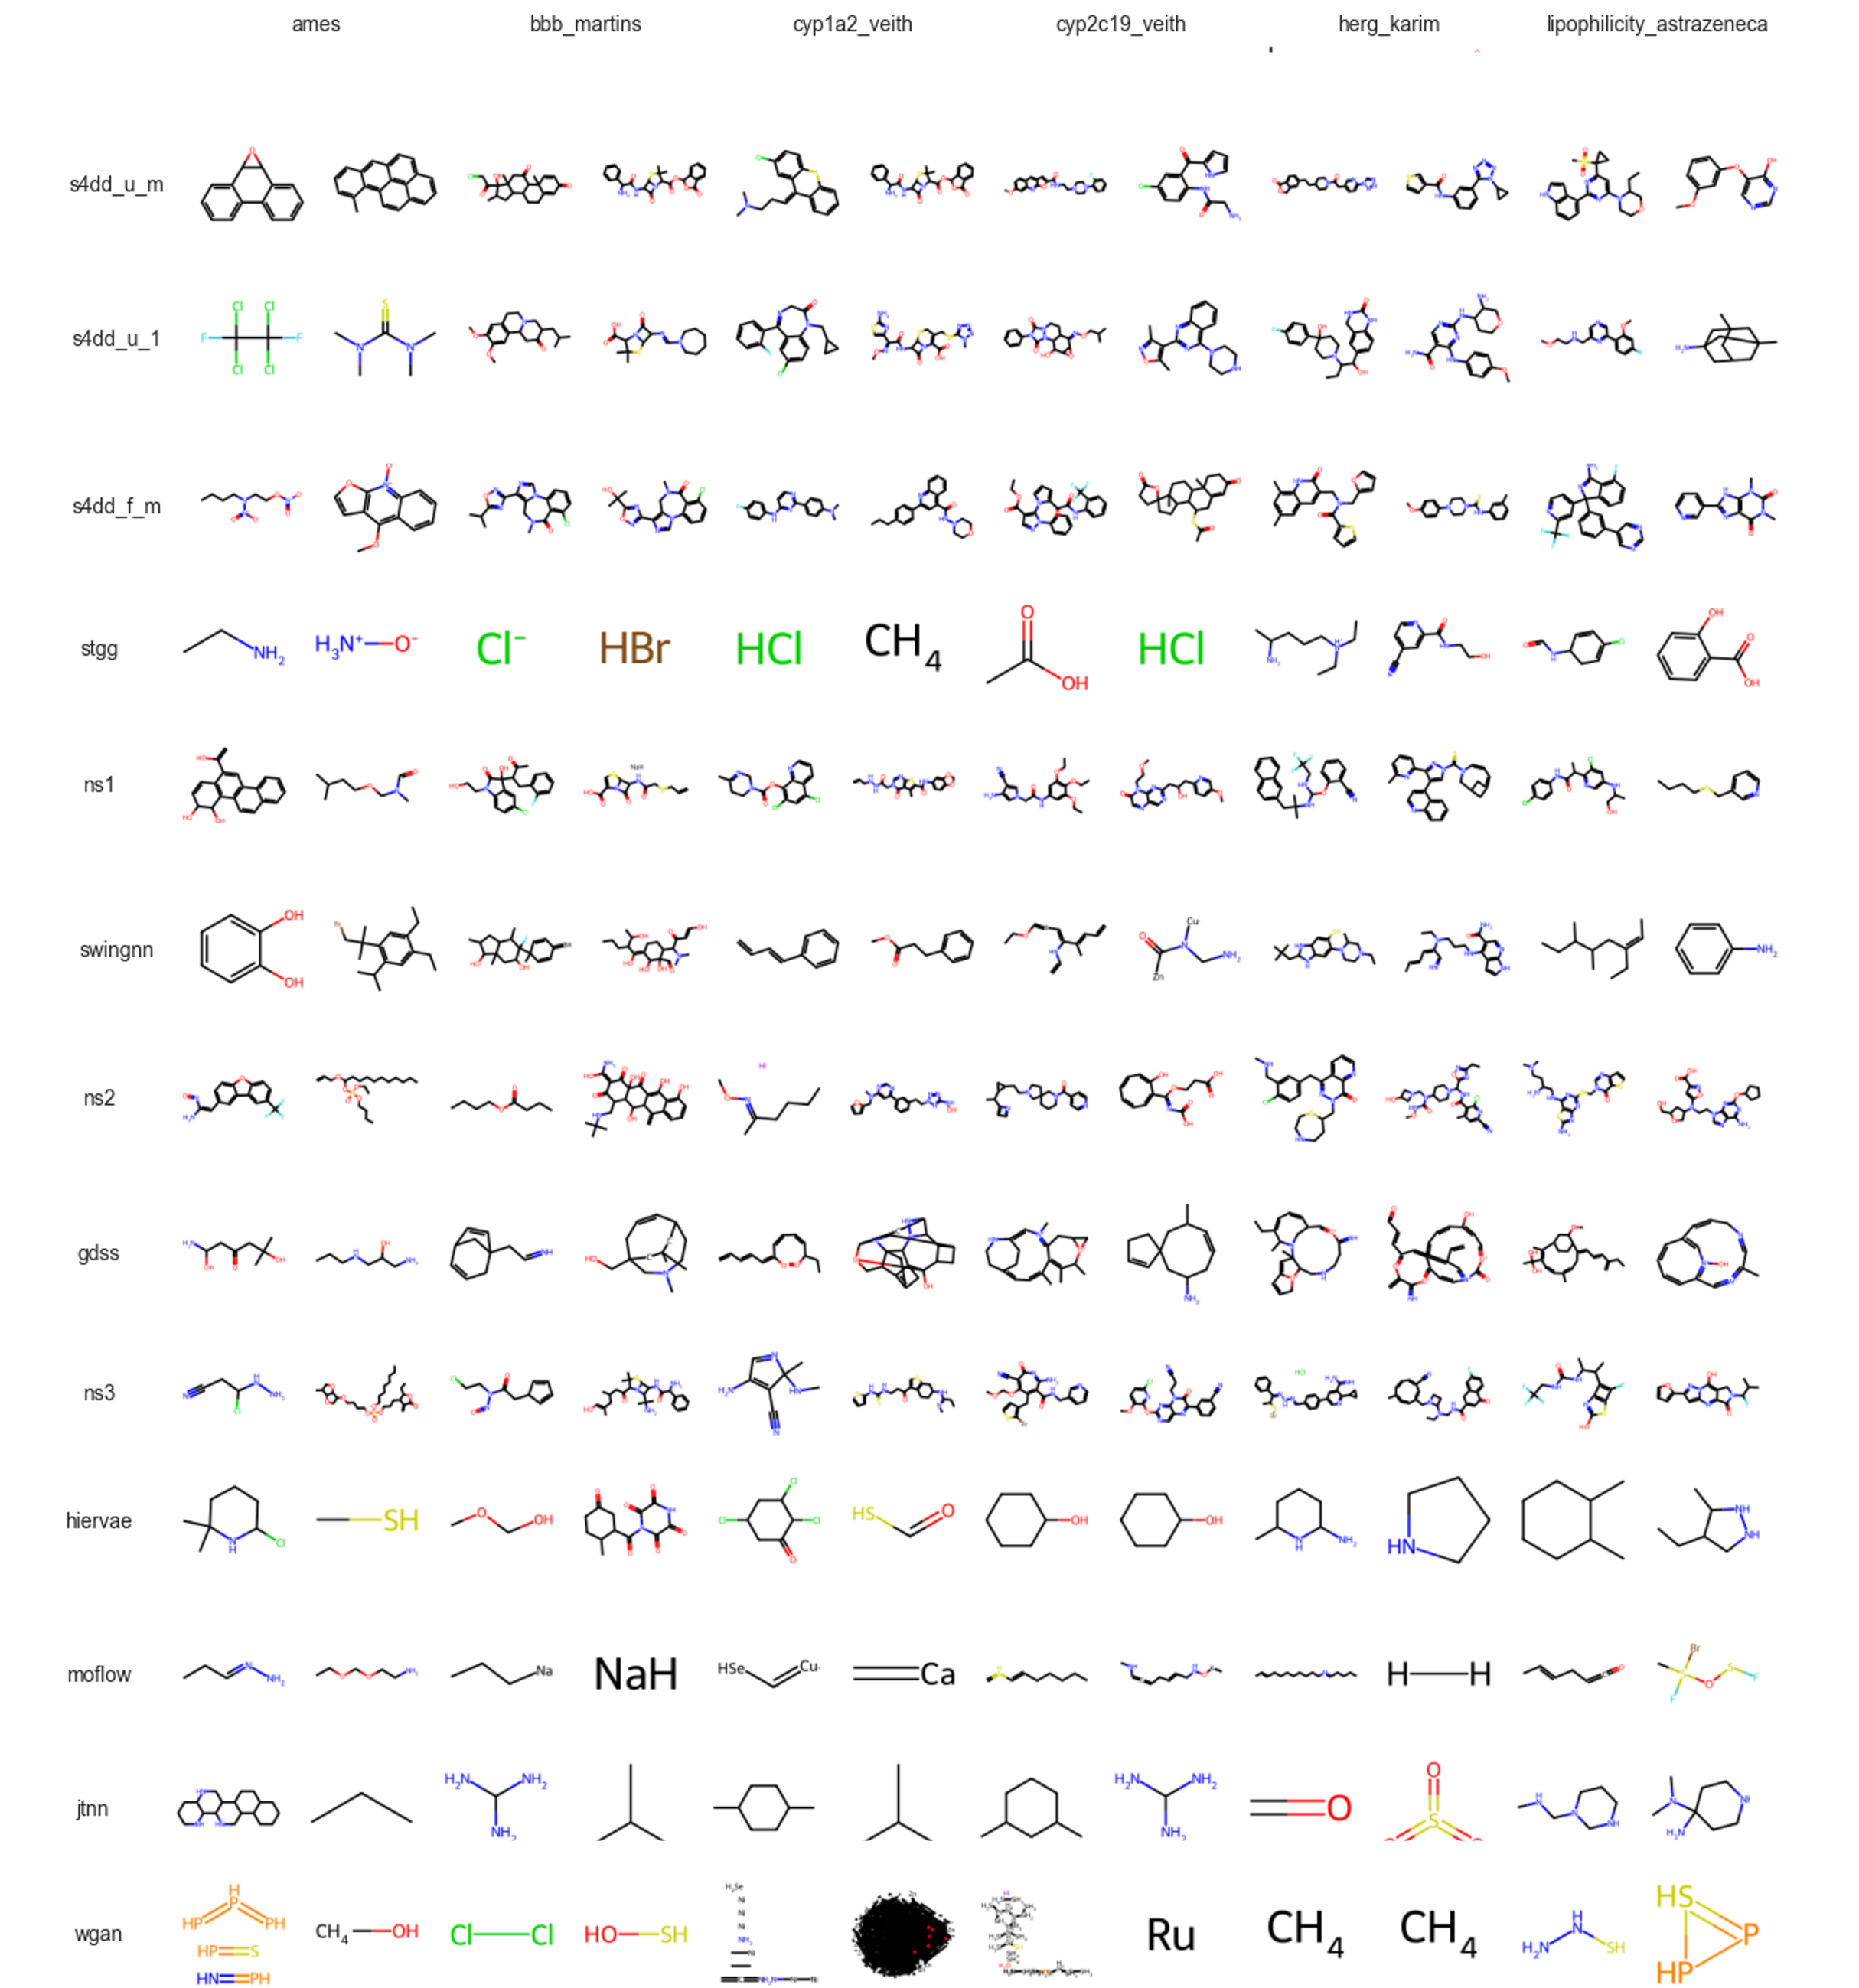
\includegraphics[width=\textwidth]{images/rankgen/real_generators/generated_molecules.png}
    \caption{Examples of molecules generated by different models across the six datasets. Each row is a generator; each dataset contributes a positive and a negative sample.}
    \label{fig:generated_molecules}
\end{figure}

\begin{figure}[H]
  \centering
  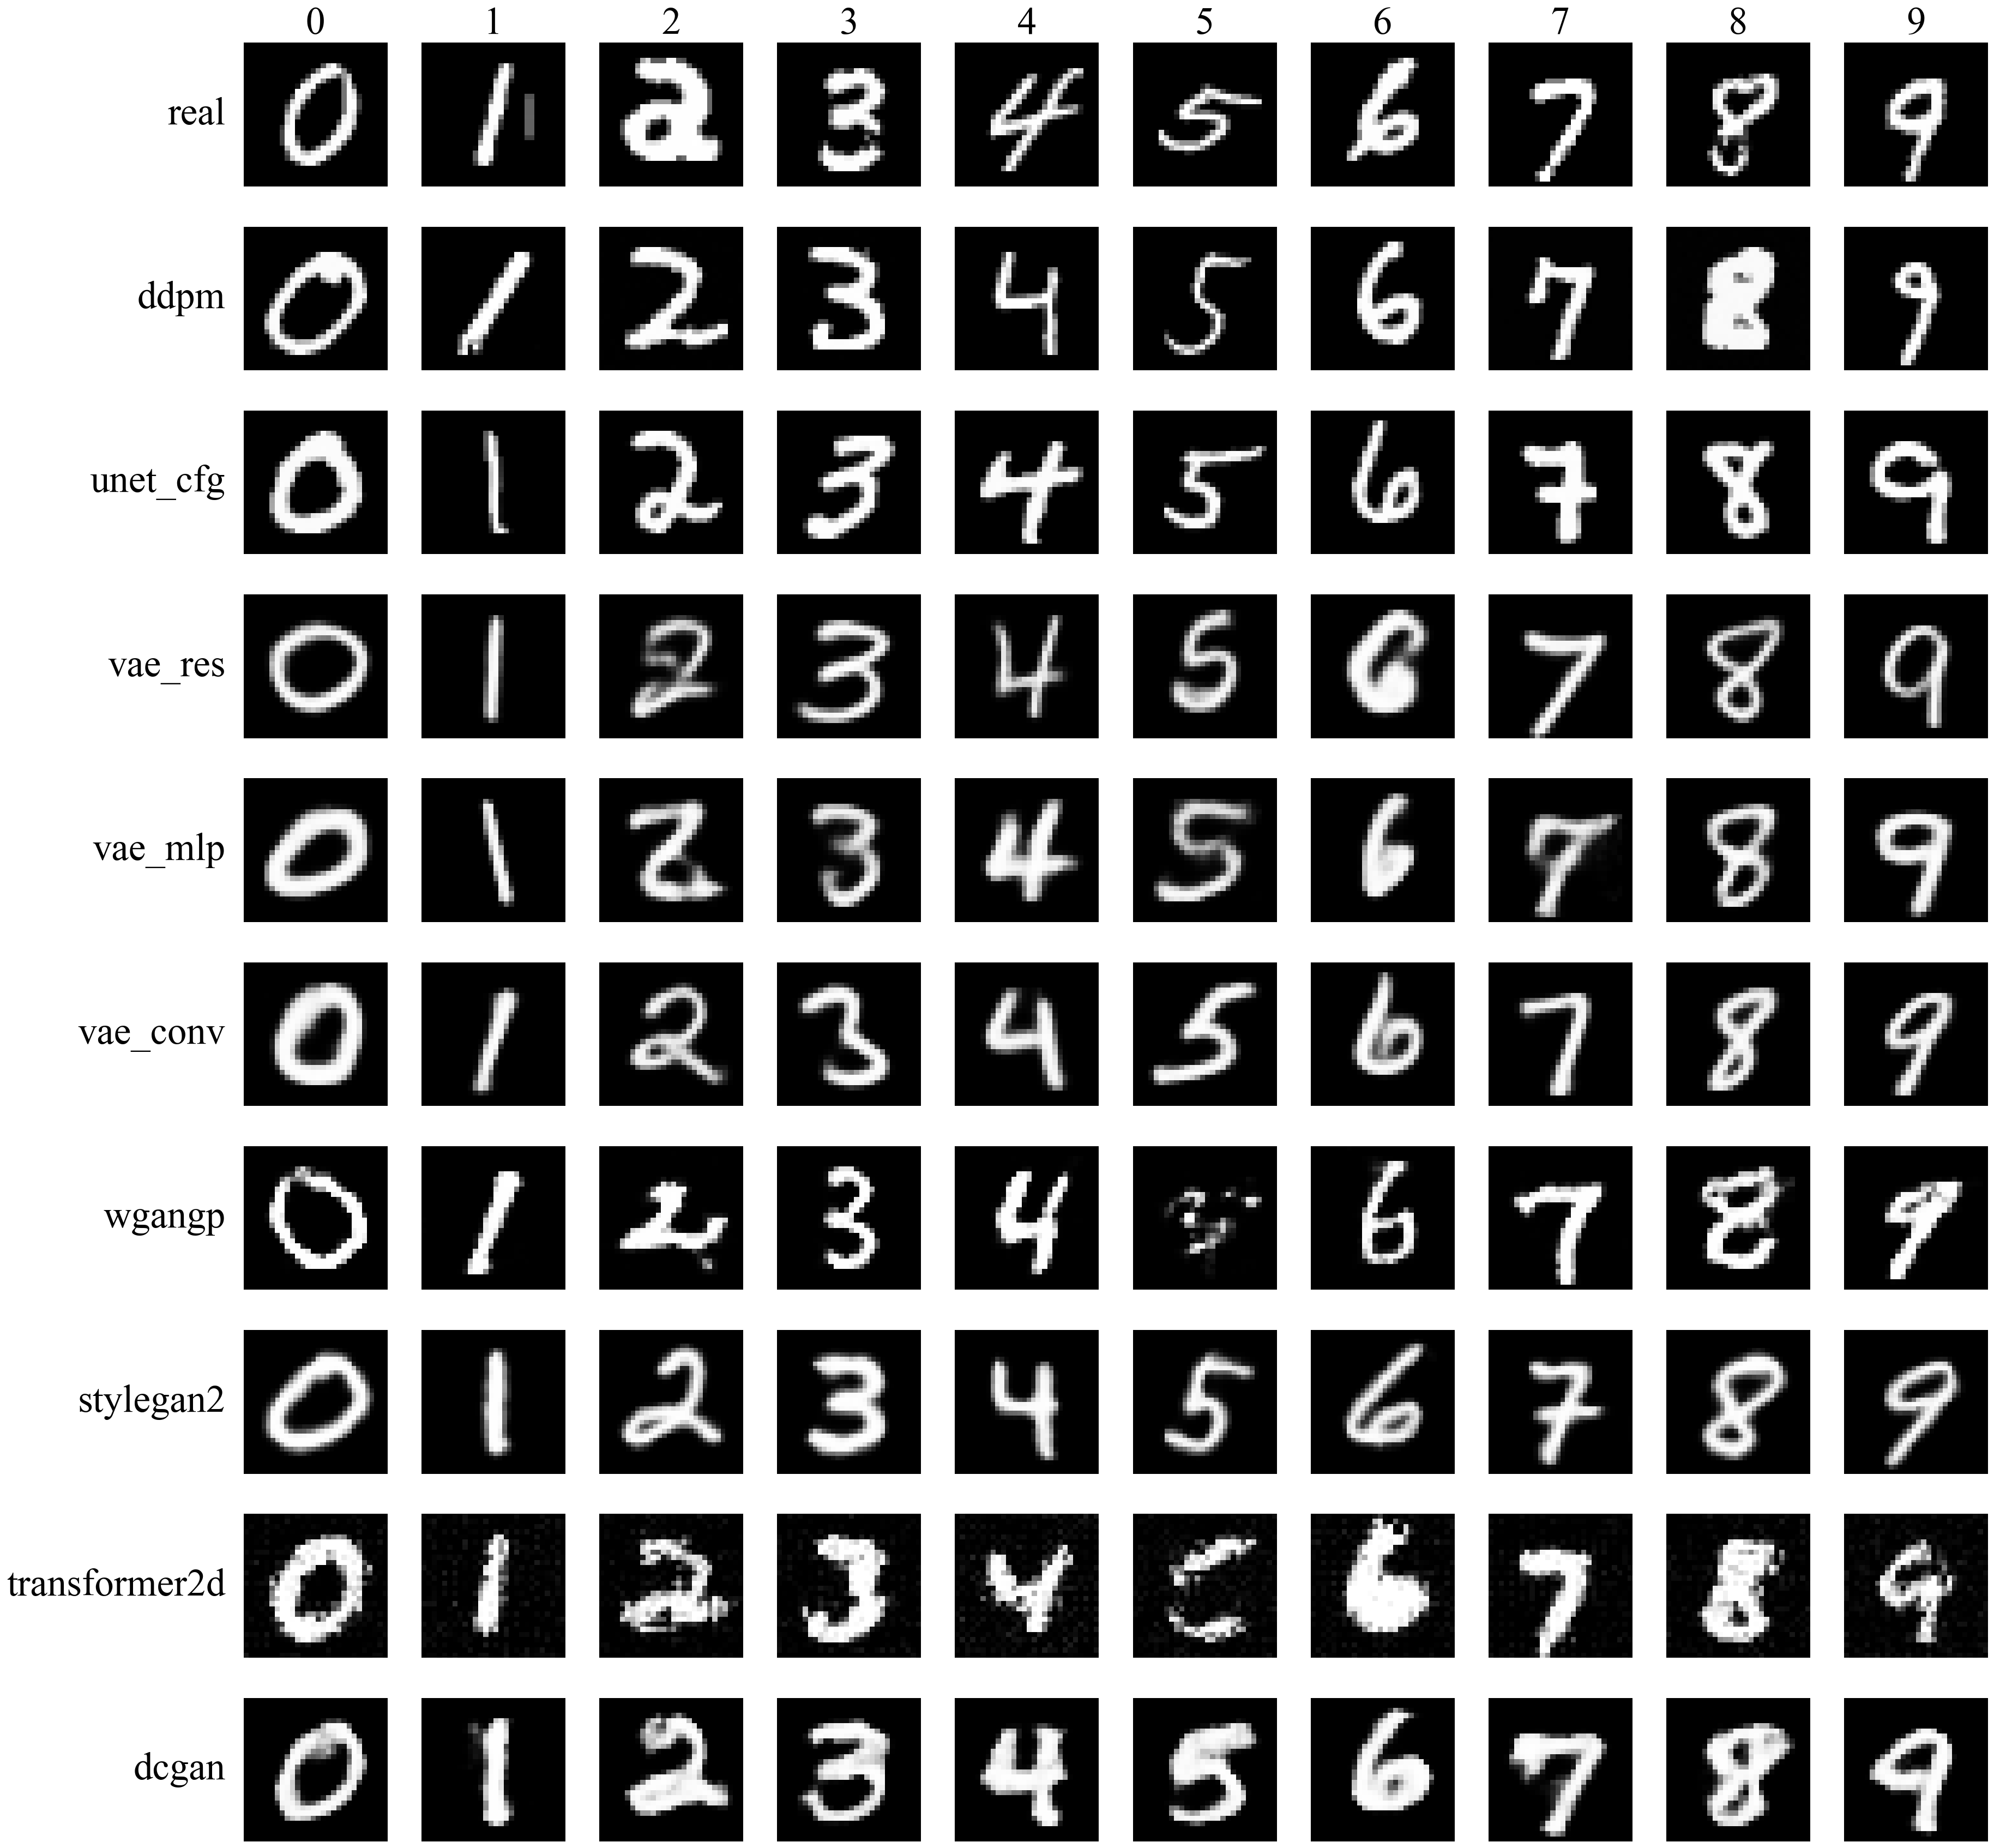
\includegraphics[width=\textwidth]{images/rankgen/real_generators/mnist_train1_generators_panel.png}
  \caption{Samples generated by each model on \textbf{MNIST}. Rows: generators; columns: class-conditional samples (uncurated).}
  \label{fig:mnist_generated_panel}
\end{figure}

\begin{figure}[H]
  \centering
  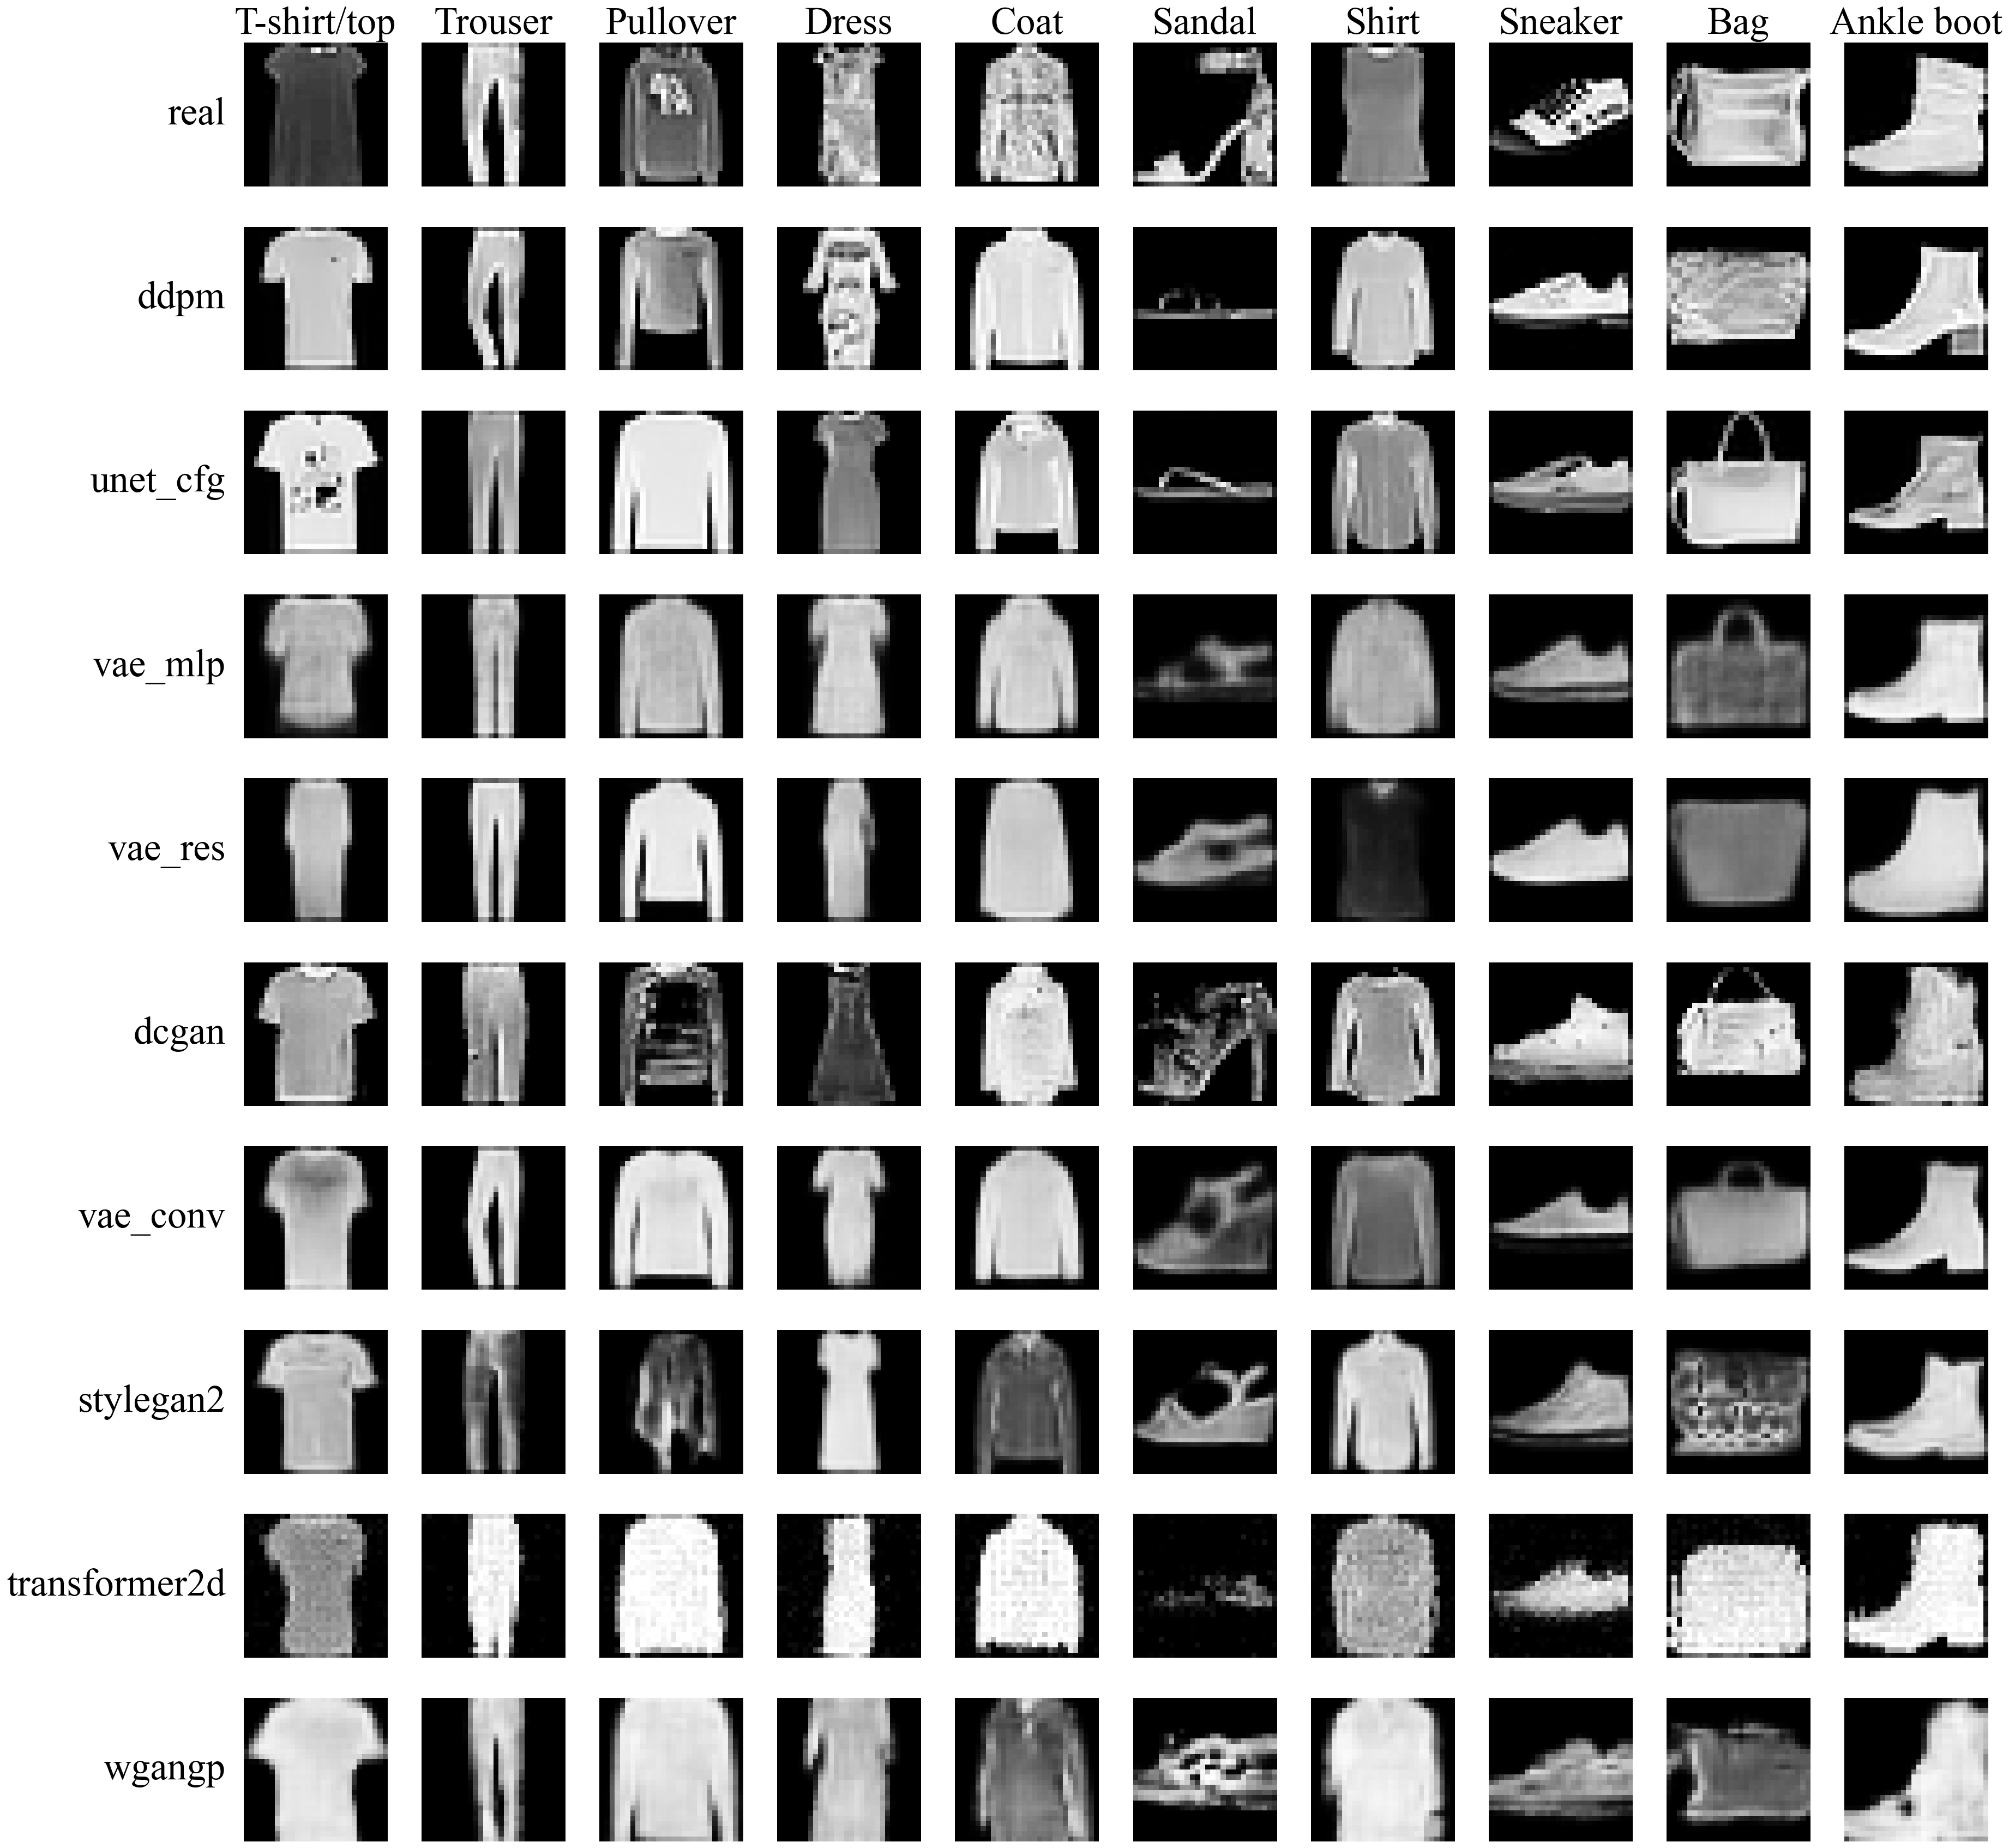
\includegraphics[width=\textwidth]{images/rankgen/real_generators/fashionmnist_train1_generators_panel.png}
  \caption{Samples generated by each model on \textbf{Fashion\textendash MNIST}. Rows: generators; columns: class-conditional samples (uncurated).}
  \label{fig:fashionmnist_generated_panel}
\end{figure}

\begin{figure}[H]
  \centering
  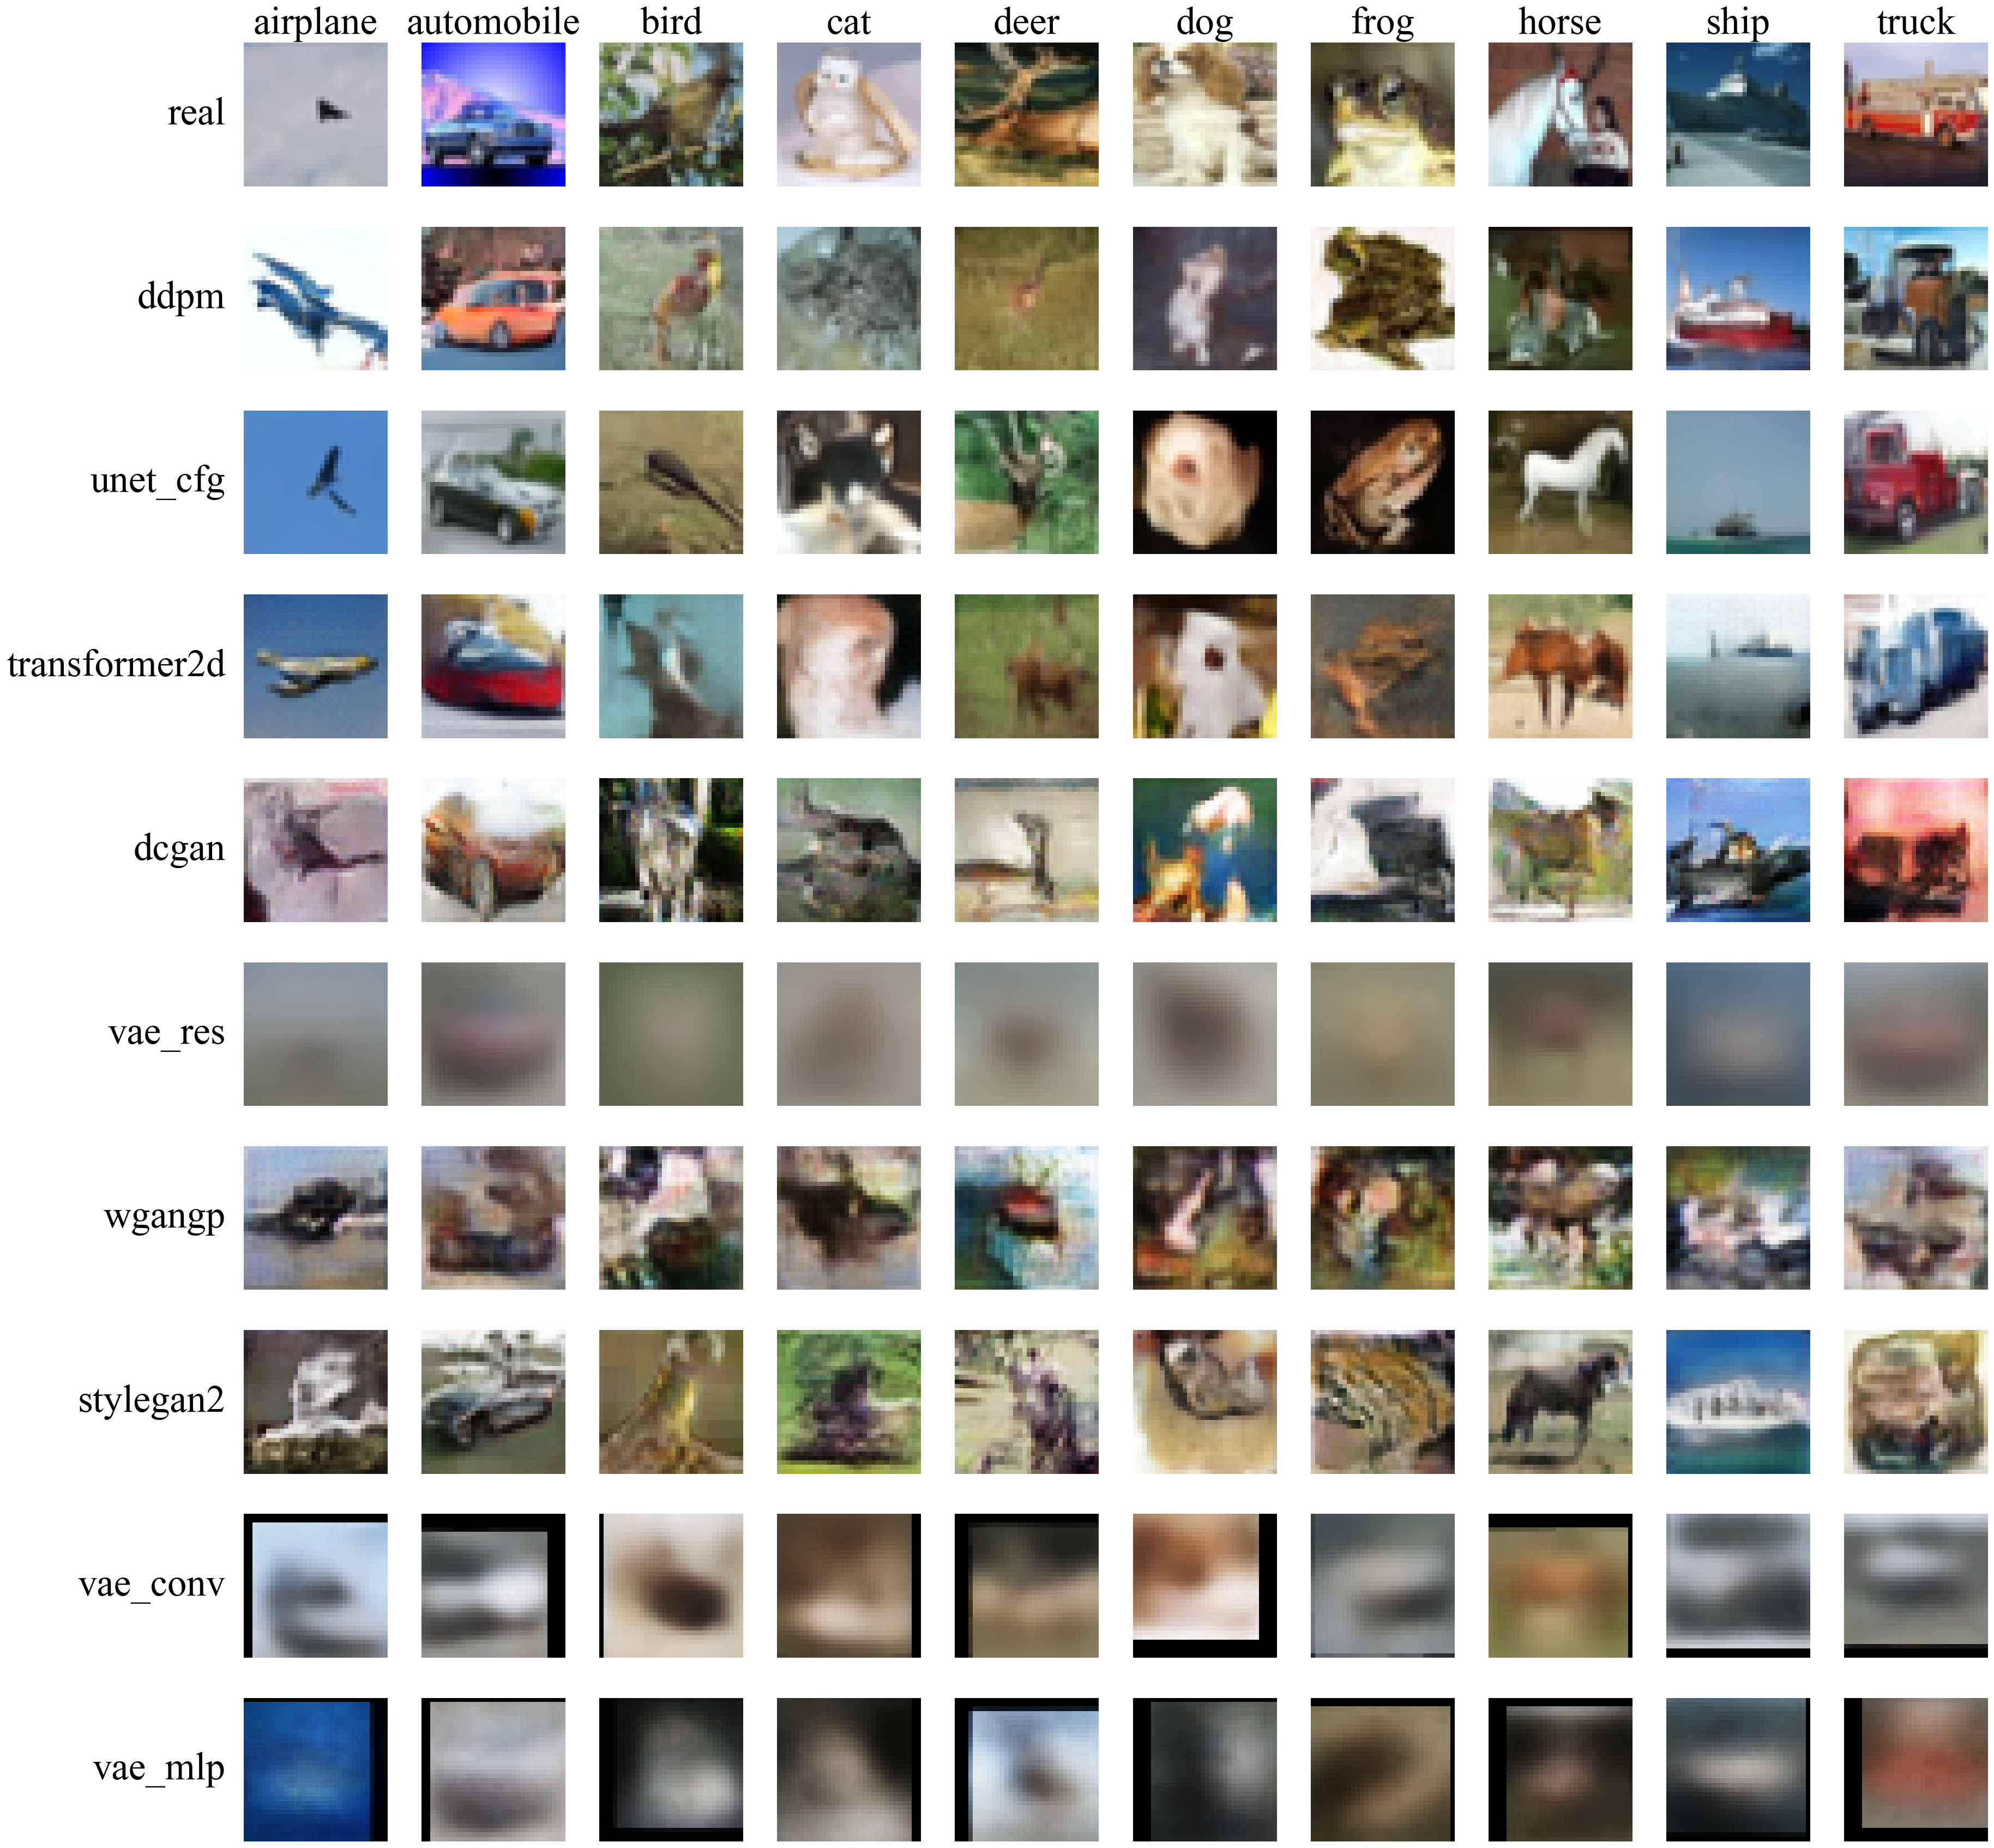
\includegraphics[width=\textwidth]{images/rankgen/real_generators/cifar10_train1_generators_panel.png}
  \caption{Samples generated by each model on \textbf{CIFAR\textendash 10}. Rows: generators; columns: per-class conditional samples (uncurated).}
  \label{fig:cifar10_generated_panel}
\end{figure}

\section{Precision, Recall, Density, and Coverage Rank of Real Generators}
\label{appendix:pr_dc_alternative_rank}
\begin{figure}[H]
  \centering
  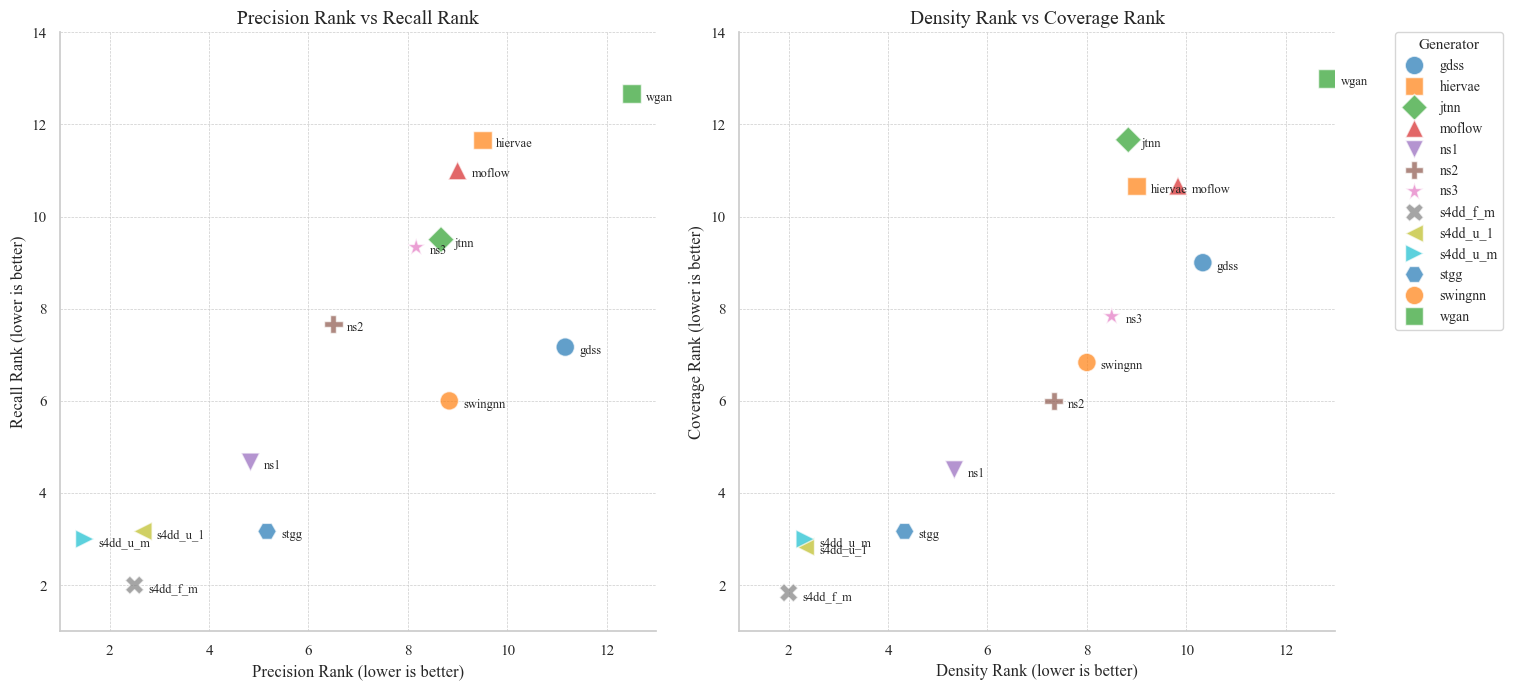
\includegraphics[width=0.75\linewidth]{images/rankgen/real_generators/generators_rank_pr.png}
  \caption{Rank comparisons of real graph generators: Precision vs.\ Recall (left) and Density vs.\ Coverage (right). Lower rank is better.}
  \label{fig:rank_pr_dc}
\end{figure}

\section{Robustness of Alternative Metrics to Data Perturbations}
\label{appendix:pr_dc}
\begin{figure}[H]
  \centering
  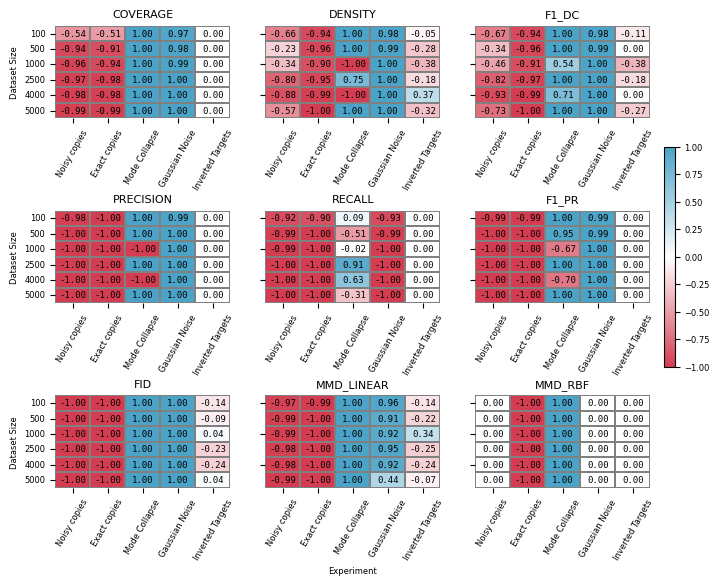
\includegraphics[width=1.0\linewidth]{images/rankgen/synthetic/pr_dc_1.png}
  \caption{Effect of perturbations on Coverage, Density, F1-DC, Precision, Recall, F1-PR, FID, MMD\_Linear, MMD\_RBF across dataset sizes.}
  \label{fig:metric_pr_dc_perturb}
\end{figure}

Despite broad use, many alternative metrics show limited robustness to perturbations; e.g., MMD\_RBF is nearly unchanged under noisy copies.

\section{Real-World Dataset Generation Experiments in Detail}
\section{Average Rank per Dataset for Each Vectorizer}

\subsection{AMES}
\begin{figure}[H]
  \centering
  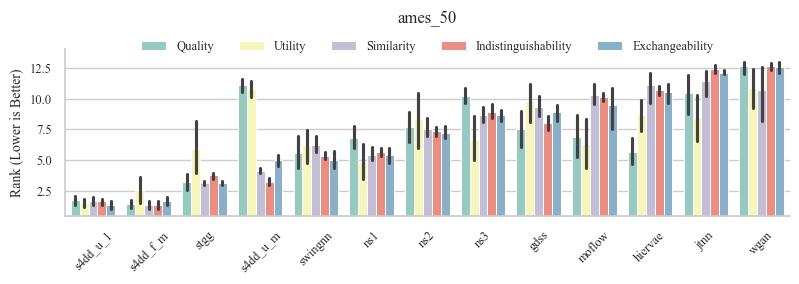
\includegraphics[width=1.0\linewidth]{images/rankgen/real_generators/generators_rank_ames.png}
  \caption{Average generator rank on \textbf{AMES} across vectorizers (lower is better).}
  \label{fig:rank_ames}
\end{figure}

\subsection{BBB Martins}
\begin{figure}[H]
  \centering
  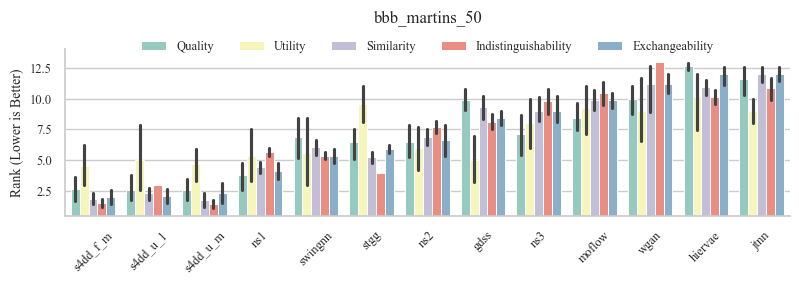
\includegraphics[width=1.0\linewidth]{images/rankgen/real_generators/generators_rank_bbb_martins.png}
  \caption{Average generator rank on \textbf{BBB Martins} across vectorizers (lower is better).}
  \label{fig:rank_bbb}
\end{figure}

\subsection{CYP1A2}
\begin{figure}[H]
  \centering
  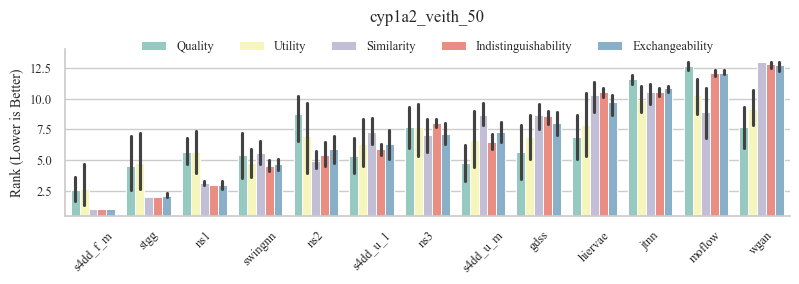
\includegraphics[width=1.0\linewidth]{images/rankgen/real_generators/generators_rank_cyp1a2.png}
  \caption{Average generator rank on \textbf{CYP1A2} across vectorizers (lower is better).}
  \label{fig:rank_cypa12}
\end{figure}

\subsection{CYP2C19}
\begin{figure}[H]
  \centering
  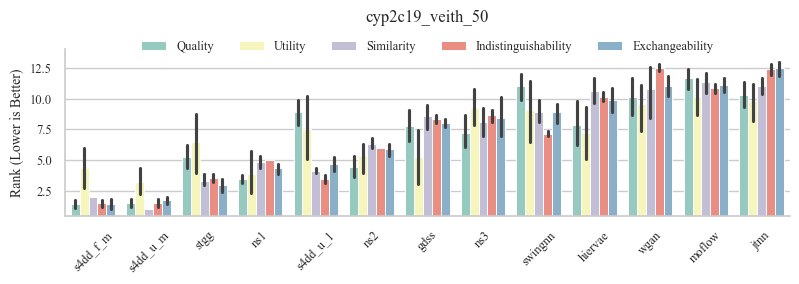
\includegraphics[width=1.0\linewidth]{images/rankgen/real_generators/generators_rank_cyp2c19.png}
  \caption{Average generator rank on \textbf{CYP2C19} across vectorizers (lower is better).}
  \label{fig:rank_cyp2c19}
\end{figure}

\subsection{hERG Karim}
\begin{figure}[H]
  \centering
  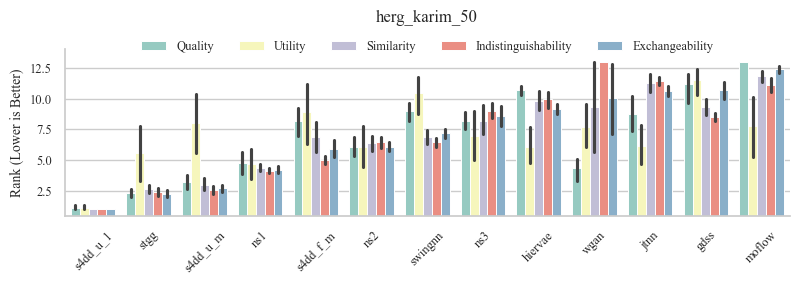
\includegraphics[width=1.0\linewidth]{images/rankgen/real_generators/generators_rank_herk_karim.png}
  \caption{Average generator rank on \textbf{hERG Karim} across vectorizers (lower is better).}
  \label{fig:rank_herg_karim}
\end{figure}

\subsection{Lipophilicity AstraZeneca}

\begin{figure}[htbp] % safer than [H]
  \centering
  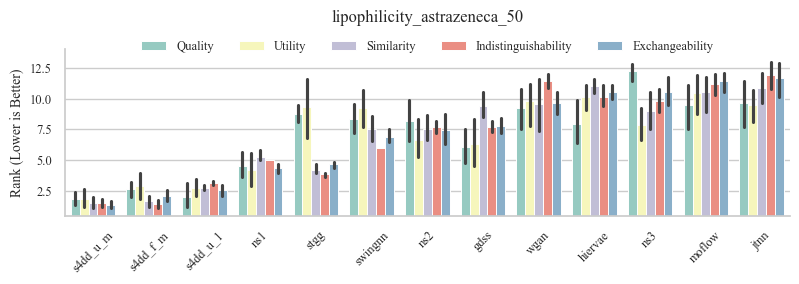
\includegraphics[width=\linewidth]{images/rankgen/real_generators/generators_rank_lipo.png}
  \caption{Average generator rank on \textbf{Lipophilicity AstraZeneca} across vectorizers (lower is better).}
  \label{fig:rank_Lipophilicity_Astrazeneca}
\end{figure}
\section{Image-Domain Experiments: Datasets, Models, and Full Results}
\label{app:image-experiments}
% (Shared preprocessing and split policy retained.)

\section{Datasets, Preprocessing, and Splits}
\label{app:image-data}
\begin{table}[H]
\centering
\scriptsize
\caption{Shared preprocessing and canonical splits used for all models and experiments.}
\label{tab:img-data-shared}
\begin{adjustbox}{max width=\linewidth}
\begin{tabular}{@{}lcccc@{}}
\toprule
Dataset & Shape $(C\times H\times W)$ & Pixel scale & Default train aug. & Split policy \\
\midrule
MNIST & $1\times28\times28$ & $[-1,1]$ from $[0,1]$ & none & stratified 50/50 \texttt{train1}/\texttt{train2} (seed 42); test untouched \\
FashionMNIST & $1\times28\times28$ & $[-1,1]$ & none & same \\
CIFAR-10 & $3\times32\times32$ & $[-1,1]$ & none$^\dagger$ & same \\
\bottomrule
\end{tabular}
\end{adjustbox}

\vspace{2pt}\footnotesize $^\dagger$ Some models enable flip/crop at training time; exports match dataset size.
\end{table}

% (Model/training tables retained; minor wording normalized.)

\section{Image Data Full Metric Results Tables}
\label{app:image-results}

% --- CIFAR-10 ---
\begin{table}[H]\centering\scriptsize
\caption{Metric values (left) and ranks (right) on \textbf{CIFAR-10}. Lower rank is better.}
\label{tab:vals-ranks-cifar10}
\begin{tabular}{l rr rr rr rr rr}
\toprule
\multirow{2}{*}{\textbf{Generator}} & \multicolumn{2}{c}{\textbf{Q}} & \multicolumn{2}{c}{\textbf{U}} & \multicolumn{2}{c}{\textbf{S}} & \multicolumn{2}{c}{\textbf{I}} & \multicolumn{2}{c}{\textbf{E}} \\
 & \textit{val} & \textit{rank} & \textit{val} & \textit{rank} & \textit{val} & \textit{rank} & \textit{val} & \textit{rank} & \textit{val} & \textit{rank} \\
\midrule
DCGAN & 0.670 & 9.0 & 0.000 & 6.5 & 0.450 & 4.0 & 0.450 & 1.0 & 0.150 & 4.0 \\
DDPM & 0.940 & 2.5 & 0.250 & 3.0 & 0.550 & 1.0 & 0.430 & 2.0 & 0.290 & 1.0 \\
StyleGAN2 & 0.880 & 4.0 & 0.000 & 6.5 & 0.190 & 9.0 & 0.080 & 6.0 & 0.060 & 7.0 \\
Transformer2D & 0.950 & 1.0 & 0.290 & 1.0 & 0.510 & 3.0 & 0.400 & 4.0 & 0.280 & 3.0 \\
UNet\_CFG & 0.940 & 2.5 & 0.250 & 2.0 & 0.530 & 2.0 & 0.410 & 3.0 & 0.280 & 2.0 \\
VAE\_Conv & 0.760 & 6.0 & 0.000 & 6.5 & 0.230 & 7.0 & 0.010 & 7.5 & 0.050 & 8.0 \\
VAE\_MLP & 0.740 & 7.0 & 0.000 & 6.5 & 0.210 & 8.0 & 0.010 & 7.5 & 0.040 & 9.0 \\
VAE\_Res & 0.770 & 5.0 & 0.000 & 6.5 & 0.400 & 5.0 & 0.000 & 9.0 & 0.080 & 5.5 \\
WGAN-GP & 0.720 & 8.0 & 0.000 & 6.5 & 0.280 & 6.0 & 0.140 & 5.0 & 0.080 & 5.5 \\
\bottomrule
\end{tabular}
\end{table}

% --- Fashion-MNIST ---
\begin{table}[H]\centering\scriptsize
\caption{Metric values (left) and ranks (right) on \textbf{Fashion-MNIST}. Lower rank is better.}
\label{tab:vals-ranks-fashionmnist}
\begin{tabular}{l rr rr rr rr rr}
\toprule
\multirow{2}{*}{\textbf{Generator}} & \multicolumn{2}{c}{\textbf{Q}} & \multicolumn{2}{c}{\textbf{U}} & \multicolumn{2}{c}{\textbf{S}} & \multicolumn{2}{c}{\textbf{I}} & \multicolumn{2}{c}{\textbf{E}} \\
 & \textit{val} & \textit{rank} & \textit{val} & \textit{rank} & \textit{val} & \textit{rank} & \textit{val} & \textit{rank} & \textit{val} & \textit{rank} \\
\midrule
DCGAN & 0.930 & 5.5 & 0.020 & 1.0 & 0.300 & 6.0 & 0.100 & 3.0 & 0.090 & 5.5 \\
DDPM & 0.940 & 2.5 & 0.000 & 5.5 & 0.500 & 1.5 & 0.170 & 1.0 & 0.160 & 1.0 \\
StyleGAN2 & 0.940 & 2.5 & 0.000 & 5.5 & 0.220 & 7.0 & 0.000 & 7.0 & 0.050 & 7.0 \\
Transformer2D & 0.810 & 8.0 & 0.000 & 5.5 & 0.060 & 8.0 & 0.000 & 7.0 & 0.010 & 8.5 \\
UNet\_CFG & 0.940 & 2.5 & 0.000 & 5.5 & 0.500 & 1.5 & 0.140 & 2.0 & 0.150 & 2.0 \\
VAE\_Conv & 0.920 & 7.0 & 0.000 & 5.5 & 0.400 & 5.0 & 0.000 & 7.0 & 0.090 & 5.5 \\
VAE\_MLP & 0.940 & 2.5 & 0.000 & 5.5 & 0.430 & 3.5 & 0.000 & 7.0 & 0.100 & 3.5 \\
VAE\_Res & 0.930 & 5.5 & 0.000 & 5.5 & 0.430 & 3.5 & 0.000 & 7.0 & 0.100 & 3.5 \\
WGAN-GP & 0.790 & 9.0 & 0.000 & 5.5 & 0.050 & 9.0 & 0.010 & 4.0 & 0.010 & 8.5 \\
\bottomrule
\end{tabular}
\end{table}
% ===== MNIST =====
\begin{table}[h]\centering\scriptsize
\caption{Metric values (left) and ranks (right) on \textbf{MNIST}. Lower rank is better.}
\label{tab:vals-ranks-mnist}
\begin{tabular}{l rr rr rr rr rr}
\toprule
\multirow{2}{*}{\textbf{Generator}} & \multicolumn{2}{c}{\textbf{Q}} & \multicolumn{2}{c}{\textbf{U}} & \multicolumn{2}{c}{\textbf{S}} & \multicolumn{2}{c}{\textbf{I}} & \multicolumn{2}{c}{\textbf{E}} \\
 & \textit{val} & \textit{rank} & \textit{val} & \textit{rank} & \textit{val} & \textit{rank} & \textit{val} & \textit{rank} & \textit{val} & \textit{rank} \\
\midrule
dcgan         & 0.560 & 9.0 & 0.000 & 7.0 & 0.010 & 9.0 & 0.000 & 6.0 & 0.000 & 9.0 \\
ddpm          & 0.970 & 3.0 & 0.000 & 7.0 & 0.570 & 2.0 & 0.130 & 1.5 & 0.170 & 1.5 \\
stylegan2     & 0.920 & 7.0 & 0.090 & 1.0 & 0.090 & 7.0 & 0.060 & 6.0 & 0.020 & 7.0 \\
transformer2d & 0.820 & 8.0 & 0.000 & 7.0 & 0.070 & 8.0 & 0.000 & 6.0 & 0.020 & 8.0 \\
unet\_cfg     & 0.970 & 3.0 & 0.000 & 7.0 & 0.580 & 1.0 & 0.130 & 1.5 & 0.170 & 1.5 \\
vae\_conv     & 0.960 & 6.0 & 0.000 & 7.0 & 0.480 & 5.0 & 0.000 & 6.0 & 0.110 & 5.0 \\
vae\_mlp      & 0.970 & 3.0 & 0.000 & 7.0 & 0.490 & 4.0 & 0.000 & 6.0 & 0.120 & 4.0 \\
vae\_res      & 0.970 & 3.0 & 0.000 & 4.0 & 0.520 & 3.0 & 0.000 & 6.0 & 0.130 & 3.0 \\
wgangp        & 0.970 & 3.0 & 0.090 & 2.0 & 0.400 & 6.0 & 0.000 & 6.0 & 0.110 & 6.0 \\
\bottomrule
\end{tabular}
\end{table}

% --- CIFAR-10 (FID/KID/PR/IS) ---
\begin{table}[H]
\centering
\small
\caption{CIFAR-10 metrics with per-metric ranks ($r{=}1$ best). $n_{\text{ref}}{=}25{,}000$, $n_{\text{gen}}{=}25{,}000$.}
\label{tab:cifar10-ranked}
\begin{tabular}{lrrrrrrrrrrrr}
\toprule
\textbf{Model} & \textbf{FID} $\downarrow$ & \textbf{r} & \textbf{KID} $\downarrow$ & \textbf{r} & \textbf{P} & \textbf{r} & \textbf{R} & \textbf{r} & \textbf{F1\_pr} & \textbf{r} & \textbf{IS} & \textbf{r} \\
\midrule
DCGAN         & 21.62 & 5 & 0.0171 & 5 & 0.165 & 6 & 0.078 & 3 & 0.106 & 3 & 2.041 & 1 \\
DDPM          &  6.67 & 1 & 0.0030 & 1 & 0.224 & 3 & 0.122 & 1 & 0.158 & 1 & 2.017 & 2 \\
StyleGAN2     & 19.26 & 3 & 0.0129 & 3 & 0.220 & 4 & 0.002 & 6 & 0.005 & 6 & 1.958 & 3 \\
UNet\_CFG     &  9.62 & 2 & 0.0069 & 2 & 0.288 & 1 & 0.093 & 2 & 0.141 & 2 & 1.944 & 4 \\
Transformer2D & 20.13 & 4 & 0.0150 & 4 & 0.286 & 2 & 0.065 & 4 & 0.106 & 3 & 1.763 & 5 \\
VAE\_Conv     & 182.67 & 7 & 0.1905 & 7 & 0.110 & 7 & 0.000 & 7 & 0.000 & 7 & 1.293 & 7 \\
VAE\_MLP      & 206.49 & 8 & 0.2182 & 8 & 0.094 & 8 & 0.000 & 7 & 0.000 & 7 & 1.280 & 8 \\
VAE\_Res      & 374.51 & 9 & 0.4439 & 9 & 0.002 & 9 & 0.000 & 7 & 0.000 & 7 & 1.006 & 9 \\
WGAN-GP        &  42.62 & 6 & 0.0342 & 6 & 0.207 & 5 & 0.017 & 5 & 0.032 & 5 & 1.652 & 6 \\
\bottomrule
\end{tabular}
\end{table}

% --- Fashion-MNIST (FID/KID/PR/IS) ---
\begin{table}[H]
\centering
\small
\caption{Fashion-MNIST metrics with per-metric ranks ($r{=}1$ best). $n_{\text{ref}}{=}30{,}000$, $n_{\text{gen}}{=}30{,}000$.}
\label{tab:fashionmnist-ranked}
\begin{tabular}{lrrrrrrrrrrrr}
\toprule
\textbf{Model} & \textbf{FID} $\downarrow$ & \textbf{r} & \textbf{KID} $\downarrow$ & \textbf{r} & \textbf{P} & \textbf{r} & \textbf{R} & \textbf{r} & \textbf{F1\_pr} & \textbf{r} & \textbf{IS} & \textbf{r} \\
\midrule
DCGAN         & 0.19 & 1 & 0.0106 & 4 & 0.215 & 7 & 0.174 & 3 & 0.192 & 3 & 2.364 & 1 \\
DDPM          & 0.71 & 2 & 0.0018 & 1 & 0.369 & 2 & 0.246 & 1 & 0.295 & 1 & 1.994 & 3 \\
StyleGAN2     & 1.45 & 4 & 0.0077 & 3 & 0.318 & 3 & 0.001 & 8 & 0.002 & 8 & 1.869 & 5 \\
UNet\_CFG     & 1.10 & 3 & 0.0042 & 2 & 0.463 & 1 & 0.188 & 2 & 0.268 & 2 & 1.905 & 4 \\
Transformer2D & 5.45 & 9 & 0.0587 & 9 & 0.090 & 8 & 0.001 & 8 & 0.002 & 8 & 1.570 & 9 \\
VAE\_Conv     & 3.82 & 6 & 0.0231 & 6 & 0.230 & 6 & 0.009 & 4 & 0.017 & 4 & 1.692 & 6 \\
VAE\_MLP      & 4.59 & 8 & 0.0216 & 5 & 0.252 & 5 & 0.007 & 5 & 0.014 & 5 & 1.677 & 7 \\
VAE\_Res      & 3.99 & 7 & 0.0257 & 7 & 0.257 & 4 & 0.006 & 6 & 0.011 & 6 & 1.673 & 8 \\
WGAN-GP        & 2.19 & 5 & 0.0423 & 8 & 0.057 & 9 & 0.005 & 7 & 0.009 & 7 & 2.013 & 2 \\
\bottomrule
\end{tabular}
\end{table}

% --- MNIST (FID/KID/PR/IS) ---
\begin{table}[H]
\centering
\small
\caption{MNIST metrics with per-metric ranks ($r{=}1$ best). $n_{\text{ref}}{=}30{,}000$, $n_{\text{gen}}{=}30{,}000$.}
\label{tab:mnist-ranked}
\begin{tabular}{lrrrrrrrrrrrr}
\toprule
\textbf{Model} & \textbf{FID} $\downarrow$ & \textbf{r} & \textbf{KID} $\downarrow$ & \textbf{r} & \textbf{P} & \textbf{r} & \textbf{R} & \textbf{r} & \textbf{F1\_pr} & \textbf{r} & \textbf{IS} & \textbf{r} \\
\midrule
DCGAN         & 3.89 & 9 & 0.0321 & 8 & 0.307 & 3 & 0.003 & 7 & 0.007 & 7 & 1.276 & 9 \\
DDPM          & 0.25 & 4 & 0.0016 & 1 & 0.488 & 2 & 0.319 & 1 & 0.386 & 1 & 1.634 & 7 \\
StyleGAN2     & 2.27 & 8 & 0.0144 & 6 & 0.291 & 4 & 0.000 & 9 & 0.000 & 9 & 1.478 & 8 \\
UNet\_CFG     & 0.29 & 5 & 0.0017 & 2 & 0.531 & 1 & 0.299 & 2 & 0.383 & 2 & 1.636 & 6 \\
Transformer2D & 0.83 & 7 & 0.1345 & 9 & 0.027 & 9 & 0.003 & 7 & 0.005 & 8 & 1.647 & 5 \\
VAE\_Conv     & 0.24 & 3 & 0.0114 & 3 & 0.223 & 5 & 0.072 & 5 & 0.109 & 5 & 1.784 & 3 \\
VAE\_MLP      & 0.23 & 2 & 0.0125 & 4 & 0.206 & 8 & 0.082 & 4 & 0.117 & 4 & 1.816 & 2 \\
VAE\_Res      & 0.40 & 6 & 0.0141 & 5 & 0.212 & 6 & 0.052 & 6 & 0.084 & 6 & 1.716 & 4 \\
WGAN-GP        & 0.14 & 1 & 0.0163 & 7 & 0.210 & 7 & 0.207 & 3 & 0.209 & 3 & 1.865 & 1 \\
\bottomrule
\end{tabular}
\end{table}

% --- Kernel-entropy diversity proxies (CIFAR-10) ---
\begin{table}[H]
\centering
\small
\caption{Kernel-entropy metrics on CIFAR-10 with per-metric ranks ($r{=}1$ best). Higher is better for RKE\_gen, FKEA-VENDI\_gen, FKEA-RKE2\_gen; lower is better for RRKE.}
\label{tab:ke-cifar10-ranked}
\begin{tabular}{lrrrrrrrrrrr}
\toprule
\textbf{Model} & $\boldsymbol{\sigma}$ & \textbf{RKE\_gen} & \textbf{r} & $\boldsymbol{\hat m}$ & \textbf{RRKE} & \textbf{r} & \textbf{FKEA-VENDI\_gen} & \textbf{r} & \textbf{FKEA-RKE2\_gen} & \textbf{r} \\
\midrule
DCGAN         & 15.18 & 0.852 & 5 & 2 & 0.179 & 5 & 13.1 & 3 & 2.3 & 3 \\
DDPM          & 15.72 & 0.942 & 1 & 3 & 0.120 & 1 & 15.7 & 1 & 2.6 & 1 \\
StyleGAN2     & 15.21 & 0.858 & 3 & 2 & 0.167 & 4 & 12.6 & 4 & 2.3 & 3 \\
UNet\_CFG     & 15.54 & 0.901 & 2 & 2 & 0.129 & 2 & 14.0 & 2 & 2.4 & 2 \\
Transformer2D & 15.28 & 0.855 & 4 & 2 & 0.165 & 3 & 12.4 & 5 & 2.4 & 2 \\
VAE\_Conv     & 15.34 & 0.335 & 7 & 1 & 0.762 & 7 &  2.8 & 7 & 1.4 & 5 \\
VAE\_MLP      & 15.54 & 0.305 & 8 & 1 & 0.829 & 8 &  2.5 & 8 & 1.4 & 5 \\
VAE\_Res      & 17.04 & 0.014 & 9 & 1 & 1.228 & 9 &  1.1 & 9 & 1.0 & 6 \\
WGAN-GP        & 14.82 & 0.745 & 6 & 2 & 0.249 & 6 &  9.5 & 6 & 2.1 & 4 \\
\bottomrule
\end{tabular}
\end{table}

% --- Kernel-entropy diversity proxies (Fashion-MNIST) ---
\begin{table}[H]
\centering
\small
\caption{Kernel-entropy metrics on Fashion-MNIST with per-metric ranks ($r{=}1$ best).}
\label{tab:ke-fashionmnist-ranked}
\begin{tabular}{lrrrrrrrrrrr}
\toprule
\textbf{Model} & $\boldsymbol{\sigma}$ & \textbf{RKE\_gen} & \textbf{r} & $\boldsymbol{\hat m}$ & \textbf{RRKE} & \textbf{r} & \textbf{FKEA-VENDI\_gen} & \textbf{r} & \textbf{FKEA-RKE2\_gen} & \textbf{r} \\
\midrule
DCGAN         & 16.63 & 0.953 & 1 & 3 & 0.120 & 3 & 14.7 & 1 & 2.6 & 1 \\
DDPM          & 16.56 & 0.945 & 2 & 3 & 0.083 & 1 & 13.1 & 2 & 2.6 & 1 \\
StyleGAN2     & 16.39 & 0.905 & 4 & 2 & 0.133 & 4 & 11.1 & 4 & 2.5 & 2 \\
UNet\_CFG     & 16.46 & 0.923 & 3 & 3 & 0.092 & 2 & 11.9 & 3 & 2.5 & 2 \\
Transformer2D & 16.62 & 0.848 & 7 & 2 & 0.357 & 9 &  8.7 & 9 & 2.3 & 4 \\
VAE\_Conv     & 16.19 & 0.852 & 6 & 2 & 0.205 & 6 &  9.3 & 6 & 2.3 & 4 \\
VAE\_MLP      & 16.26 & 0.852 & 6 & 2 & 0.199 & 5 &  9.0 & 8 & 2.3 & 4 \\
VAE\_Res      & 16.12 & 0.837 & 8 & 2 & 0.211 & 7 &  9.1 & 7 & 2.3 & 4 \\
WGAN-GP        & 16.54 & 0.879 & 5 & 2 & 0.263 & 8 & 10.6 & 5 & 2.4 & 3 \\
\bottomrule
\end{tabular}
\end{table}

% --- Kernel-entropy diversity proxies (MNIST) ---
\begin{table}[H]
\centering
\small
\caption{Kernel-entropy metrics on MNIST with per-metric ranks ($r{=}1$ best).}
\label{tab:ke-mnist-ranked}
\begin{tabular}{lrrrrrrrrrrr}
\toprule
\textbf{Model} & $\boldsymbol{\sigma}$ & \textbf{RKE\_gen} & \textbf{r} & $\boldsymbol{\hat m}$ & \textbf{RRKE} & \textbf{r} & \textbf{FKEA-VENDI\_gen} & \textbf{r} & \textbf{FKEA-RKE2\_gen} & \textbf{r} \\
\midrule
DCGAN         & 13.58 & 0.869 & 8 & 2 & 0.331 & 8 &  8.1 & 8 & 2.3 & 5 \\
DDPM          & 13.48 & 0.971 & 3 & 3 & 0.070 & 1 & 13.5 & 2 & 2.7 & 1 \\
StyleGAN2     & 13.21 & 0.882 & 7 & 2 & 0.235 & 7 &  8.7 & 7 & 2.4 & 4 \\
UNet\_CFG     & 13.40 & 0.972 & 2 & 3 & 0.071 & 2 & 13.0 & 3 & 2.6 & 2 \\
Transformer2D & 15.28 & 0.850 & 9 & 2 & 0.540 & 9 & 10.7 & 6 & 2.3 & 5 \\
VAE\_Conv     & 13.46 & 0.937 & 5 & 3 & 0.146 & 4 & 12.5 & 4 & 2.5 & 3 \\
VAE\_MLP      & 13.67 & 0.953 & 4 & 3 & 0.150 & 5 & 13.0 & 3 & 2.6 & 2 \\
VAE\_Res      & 13.38 & 0.921 & 6 & 3 & 0.161 & 6 & 11.9 & 5 & 2.5 & 3 \\
WGAN-GP        & 13.93 & 0.994 & 1 & 3 & 0.145 & 3 & 15.0 & 1 & 2.7 & 1 \\
\bottomrule
\end{tabular}
\end{table}


\paragraph{Relationship between RankGen and conventional metrics.}
Tables \ref{tab:vals-ranks-cifar10}--\ref{tab:vals-ranks-mnist}(RankGen metrics) and Tables~\ref{tab:cifar10-ranked}--\ref{tab:ke-mnist-ranked}(conventional metrics) show
that the two families of metrics agree at a coarse level but diverge in
precisely the situations where standard metrics are known to be unreliable.
Across CIFAR--10, Fashion--MNIST, and MNIST, diffusion models (DDPM, UNet--CFG)
rank near the top under both RankGen and baseline metrics such as
FID~\citep{heusel2017gans}, KID~\citep{binkowski2018demystifying},
precision/recall for distributions~\citep{sajjadi2018assessing,kynkaanniemi2019improved}
and Inception Score~\citep{salimans2016improved}, as well as
VENDI/RKE/FKEA kernel–entropy metrics~\citep{friedman2023vendi,pasarkar2024cousins,jalali2024fkea,luo2024converge}.
However, the generators that the conventional metrics disagree on are exactly
the ones where RankGen provides additional diagnostic resolution. For example,
StyleGAN2 achieves competitive FID/KID and very high precision but extremely low
recall, whereas RankGen penalizes it strongly through low Utility and low
Similarity, revealing its concentrated, mode-dropping behaviour. Conversely,
WGAN--GP obtains middling FID/KID but is classified by RankGen as having almost
zero Utility, correctly indicating that its samples add little task-relevant
information despite looking plausible in feature space. VAEs rank moderately
under FID/KID but RankGen identifies their weak task fidelity (low Quality) and
weak local mixing (low Indistinguishability), especially on CIFAR--10. Overall,
baseline metrics capture global similarity, while RankGen captures
\emph{task fidelity, augmentation value, local mixing, and copying}, explaining
the ranking discrepancies and providing complementary diagnostic information.




\section{Reproducibility Notes}
All experiments use seed $42$ unless otherwise stated. Evaluation uses equal $n_{\text{ref}}$ and $n_{\text{gen}}$ per dataset (see captions). 
